% Options for packages loaded elsewhere
\PassOptionsToPackage{unicode}{hyperref}
\PassOptionsToPackage{hyphens}{url}
\PassOptionsToPackage{space}{xeCJK}
\documentclass[
  a4paper,
]{article}
\usepackage{xcolor}
\usepackage[margin=24mm]{geometry}
\usepackage{amsmath,amssymb}
\setcounter{secnumdepth}{-\maxdimen} % remove section numbering
\usepackage{iftex}
\ifPDFTeX
  \usepackage[T1]{fontenc}
  \usepackage[utf8]{inputenc}
  \usepackage{textcomp} % provide euro and other symbols
\else % if luatex or xetex
  \usepackage{unicode-math} % this also loads fontspec
  \defaultfontfeatures{Scale=MatchLowercase}
  \defaultfontfeatures[\rmfamily]{Ligatures=TeX,Scale=1}
\fi
\usepackage{lmodern}
\ifPDFTeX\else
  % xetex/luatex font selection
  \setmonofont[]{DejaVuSansMono.ttf}
  \ifXeTeX
    \usepackage{xeCJK}
    \setCJKmainfont[]{HaranoAjiMincho-Regular.otf}
  \fi
  \ifLuaTeX
    \usepackage[]{luatexja-fontspec}
    \setmainjfont[]{HaranoAjiMincho-Regular.otf}
  \fi
\fi
% Use upquote if available, for straight quotes in verbatim environments
\IfFileExists{upquote.sty}{\usepackage{upquote}}{}
\IfFileExists{microtype.sty}{% use microtype if available
  \usepackage[]{microtype}
  \UseMicrotypeSet[protrusion]{basicmath} % disable protrusion for tt fonts
}{}
\makeatletter
\@ifundefined{KOMAClassName}{% if non-KOMA class
  \IfFileExists{parskip.sty}{%
    \usepackage{parskip}
  }{% else
    \setlength{\parindent}{0pt}
    \setlength{\parskip}{6pt plus 2pt minus 1pt}}
}{% if KOMA class
  \KOMAoptions{parskip=half}}
\makeatother
\usepackage{color}
\usepackage{fancyvrb}
\newcommand{\VerbBar}{|}
\newcommand{\VERB}{\Verb[commandchars=\\\{\}]}
\DefineVerbatimEnvironment{Highlighting}{Verbatim}{commandchars=\\\{\}}
% Add ',fontsize=\small' for more characters per line
\newenvironment{Shaded}{}{}
\newcommand{\AlertTok}[1]{\textcolor[rgb]{1.00,0.00,0.00}{\textbf{#1}}}
\newcommand{\AnnotationTok}[1]{\textcolor[rgb]{0.38,0.63,0.69}{\textbf{\textit{#1}}}}
\newcommand{\AttributeTok}[1]{\textcolor[rgb]{0.49,0.56,0.16}{#1}}
\newcommand{\BaseNTok}[1]{\textcolor[rgb]{0.25,0.63,0.44}{#1}}
\newcommand{\BuiltInTok}[1]{\textcolor[rgb]{0.00,0.50,0.00}{#1}}
\newcommand{\CharTok}[1]{\textcolor[rgb]{0.25,0.44,0.63}{#1}}
\newcommand{\CommentTok}[1]{\textcolor[rgb]{0.38,0.63,0.69}{\textit{#1}}}
\newcommand{\CommentVarTok}[1]{\textcolor[rgb]{0.38,0.63,0.69}{\textbf{\textit{#1}}}}
\newcommand{\ConstantTok}[1]{\textcolor[rgb]{0.53,0.00,0.00}{#1}}
\newcommand{\ControlFlowTok}[1]{\textcolor[rgb]{0.00,0.44,0.13}{\textbf{#1}}}
\newcommand{\DataTypeTok}[1]{\textcolor[rgb]{0.56,0.13,0.00}{#1}}
\newcommand{\DecValTok}[1]{\textcolor[rgb]{0.25,0.63,0.44}{#1}}
\newcommand{\DocumentationTok}[1]{\textcolor[rgb]{0.73,0.13,0.13}{\textit{#1}}}
\newcommand{\ErrorTok}[1]{\textcolor[rgb]{1.00,0.00,0.00}{\textbf{#1}}}
\newcommand{\ExtensionTok}[1]{#1}
\newcommand{\FloatTok}[1]{\textcolor[rgb]{0.25,0.63,0.44}{#1}}
\newcommand{\FunctionTok}[1]{\textcolor[rgb]{0.02,0.16,0.49}{#1}}
\newcommand{\ImportTok}[1]{\textcolor[rgb]{0.00,0.50,0.00}{\textbf{#1}}}
\newcommand{\InformationTok}[1]{\textcolor[rgb]{0.38,0.63,0.69}{\textbf{\textit{#1}}}}
\newcommand{\KeywordTok}[1]{\textcolor[rgb]{0.00,0.44,0.13}{\textbf{#1}}}
\newcommand{\NormalTok}[1]{#1}
\newcommand{\OperatorTok}[1]{\textcolor[rgb]{0.40,0.40,0.40}{#1}}
\newcommand{\OtherTok}[1]{\textcolor[rgb]{0.00,0.44,0.13}{#1}}
\newcommand{\PreprocessorTok}[1]{\textcolor[rgb]{0.74,0.48,0.00}{#1}}
\newcommand{\RegionMarkerTok}[1]{#1}
\newcommand{\SpecialCharTok}[1]{\textcolor[rgb]{0.25,0.44,0.63}{#1}}
\newcommand{\SpecialStringTok}[1]{\textcolor[rgb]{0.73,0.40,0.53}{#1}}
\newcommand{\StringTok}[1]{\textcolor[rgb]{0.25,0.44,0.63}{#1}}
\newcommand{\VariableTok}[1]{\textcolor[rgb]{0.10,0.09,0.49}{#1}}
\newcommand{\VerbatimStringTok}[1]{\textcolor[rgb]{0.25,0.44,0.63}{#1}}
\newcommand{\WarningTok}[1]{\textcolor[rgb]{0.38,0.63,0.69}{\textbf{\textit{#1}}}}
\usepackage{longtable,booktabs,array}
\newcounter{none} % for unnumbered tables
\usepackage{calc} % for calculating minipage widths
% Correct order of tables after \paragraph or \subparagraph
\usepackage{etoolbox}
\makeatletter
\patchcmd\longtable{\par}{\if@noskipsec\mbox{}\fi\par}{}{}
\makeatother
% Allow footnotes in longtable head/foot
\IfFileExists{footnotehyper.sty}{\usepackage{footnotehyper}}{\usepackage{footnote}}
\makesavenoteenv{longtable}
\usepackage{graphicx}
\makeatletter
\newsavebox\pandoc@box
\newcommand*\pandocbounded[1]{% scales image to fit in text height/width
  \sbox\pandoc@box{#1}%
  \Gscale@div\@tempa{\textheight}{\dimexpr\ht\pandoc@box+\dp\pandoc@box\relax}%
  \Gscale@div\@tempb{\linewidth}{\wd\pandoc@box}%
  \ifdim\@tempb\p@<\@tempa\p@\let\@tempa\@tempb\fi% select the smaller of both
  \ifdim\@tempa\p@<\p@\scalebox{\@tempa}{\usebox\pandoc@box}%
  \else\usebox{\pandoc@box}%
  \fi%
}
% Set default figure placement to htbp
\def\fps@figure{htbp}
\makeatother
\setlength{\emergencystretch}{3em} % prevent overfull lines
\providecommand{\tightlist}{%
  \setlength{\itemsep}{0pt}\setlength{\parskip}{0pt}}
\usepackage{bookmark}
\IfFileExists{xurl.sty}{\usepackage{xurl}}{} % add URL line breaks if available
\urlstyle{same}
\hypersetup{
  hidelinks,
  pdfcreator={LaTeX via pandoc}}

\author{}
\date{}

\begin{document}

\section{Preliminary Summary of Harmonic Readout and c=1 Area Sweep in
an AB Two-Body Closed Phase System
v3}\label{preliminary-summary-of-harmonic-readout-and-c1-area-sweep-in-an-ab-two-body-closed-phase-system-v3}

\textbf{Date:} 2026-07-15 \textbf{Author:} Noriaki Kihara
\textbf{Position:} Summary of the AB two-body preliminary experiment
group in the Wave Information Readout series \textbf{Version DOI:}
10.5281/zenodo.21367800 \textbf{Concept DOI:} 10.5281/zenodo.21318696

V3 applies the fermion-like recoil map to \texttt{chi\_read} as the
scattering-matrix factor \texttt{q\_out\_factor}.

\begin{center}\rule{0.5\linewidth}{0.5pt}\end{center}

\subsection{Abstract}\label{abstract}

This summary consolidates six preliminary experiments performed on an AB
two-body closed phase system. V3 keeps the same scope and claims and
incorporates a fermion-like recoil map into the same AB
acceleration-readout frame:

\begin{enumerate}
\def\labelenumi{\arabic{enumi}.}
\tightlist
\item
  one-angle circumferential phase harmonic readout,
\item
  parameter sweep of the one-angle circumferential phase harmonic
  readout,
\item
  internal \texttt{c=1} calibration and \texttt{chi-tau} area sweep,
\item
  parameter sweep of the internal \texttt{c=1} calibration,
\item
  inverse-area compensation diagnosis in the \texttt{chi-tau} plane, and
\item
  extended sweep for native inverse-area readout, and
\item
  fermion-like recoil harmonic readout protocol.
\end{enumerate}

The preceding ABC multigauge interference readout paper showed that, in
a minimal ABC closed phase system that does not place a background space
first, the measuring device itself can be defined as a complex phase
wave inside the same system, and mass-like, momentum-like, and
energy-like conserved readouts can be constructed from interference.

The present experiment group takes one step further. It verifies that an
acceleration-like readout can be represented by harmonic readout in the
AB two-body relation itself.

However, the AB two-body system alone could not determine whether the
acceleration-like readout changes with the position phase difference, or
distance, according to an inverse law or an inverse-square law.

The central achievement of this experiment group is not merely the
display of harmonic motion. No external standard force, spring equation,
gravitational equation, or Coulomb equation is introduced. No individual
forces \texttt{f\_A} and \texttt{f\_B} are introduced. Using only the
label-free two-body relation \texttt{f\_AB}, an acceleration-like
readout was constructed.

At the same time, the experiment clarified a boundary. In the AB
two-body system, the measuring device is on the measured object itself.
Therefore, although relative-distance change can be read, there is no
independent gauge that can decide whether the change follows

\begin{Shaded}
\begin{Highlighting}[]
\NormalTok{L\_AB}
\NormalTok{1 / L\_AB}
\NormalTok{1 / L\_AB\^{}2}
\end{Highlighting}
\end{Shaded}

The gauge used to measure the interval is itself affected by the same
closed phase system. Even after adding a temporal phase difference in
addition to the spatial position phase difference, and even after
imposing an internal \texttt{c=1}-like calibration to reproduce a
time-development-like effect, the conclusion did not change.

Thus, the determination of the distance exponent remains a task for a
separate ABC three-body experiment with an independent metrical gauge.

\textbf{Keywords:} AB two-body closed phase system, label-free two-arc
relative phase, harmonic readout, acceleration-like readout, c=1
internal calibration, chi-tau area, inverse-area diagnosis, native
readout

\begin{center}\rule{0.5\linewidth}{0.5pt}\end{center}

\subsection{1. Experiment List}\label{experiment-list}

{\def\LTcaptype{none} % do not increment counter
\begin{longtable}[]{@{}
  >{\raggedleft\arraybackslash}p{(\linewidth - 6\tabcolsep) * \real{0.3077}}
  >{\raggedright\arraybackslash}p{(\linewidth - 6\tabcolsep) * \real{0.2308}}
  >{\raggedright\arraybackslash}p{(\linewidth - 6\tabcolsep) * \real{0.2308}}
  >{\raggedright\arraybackslash}p{(\linewidth - 6\tabcolsep) * \real{0.2308}}@{}}
\toprule\noalign{}
\begin{minipage}[b]{\linewidth}\raggedleft
No.
\end{minipage} & \begin{minipage}[b]{\linewidth}\raggedright
Experiment
\end{minipage} & \begin{minipage}[b]{\linewidth}\raggedright
Purpose
\end{minipage} & \begin{minipage}[b]{\linewidth}\raggedright
Main result
\end{minipage} \\
\midrule\noalign{}
\endhead
\bottomrule\noalign{}
\endlastfoot
1 & One-angle harmonic readout & Test whether \texttt{D\_AB},
\texttt{V\_AB}, and \texttt{f\_AB} can be read label-free & Readable \\
2 & One-angle parameter sweep & Robustness against initial deviation,
period, and readout leakage & Harmonic oscillation detected in all
cases \\
3 & \texttt{c=1} area sweep & Separate \texttt{s} from
\texttt{tau\_read} and test whether a \texttt{chi-tau} plane stands &
Area detected under independent \texttt{tau} \\
4 & \texttt{c=1} parameter sweep & Test whether \texttt{c=1} is
sufficient for area formation & Not sufficient \\
5 & Inverse-area compensation diagnosis & Test whether
\texttt{1/A\_chi\_tau} remains natively on the closure-compensation side
& Not detected \\
6 & Native inverse-area extended sweep & Search broad conditions for
\texttt{alpha≈2} & Not detected natively \\
7 & V3 fermion-like recoil protocol & Re-test acceleration-like readout
with a recoil map near the AB center & \texttt{q\_out\_factor=-1}
applied to \texttt{chi\_read}; harmonic readout and \texttt{chi-tau}
surface maintained \\
\end{longtable}
}

\begin{center}\rule{0.5\linewidth}{0.5pt}\end{center}

\subsection{2. One-Angle Circumferential Phase Harmonic
Readout}\label{one-angle-circumferential-phase-harmonic-readout}

\subsubsection{2.1 Meaning of the
Experiment}\label{meaning-of-the-experiment}

The AB pair was read as a closed phase system without placing an
observer \texttt{C}.

The experiment did not introduce

\begin{Shaded}
\begin{Highlighting}[]
\NormalTok{f\_A}
\NormalTok{f\_B}
\end{Highlighting}
\end{Shaded}

as independent forces. It read only

\begin{Shaded}
\begin{Highlighting}[]
\NormalTok{f\_AB}
\end{Highlighting}
\end{Shaded}

as relational compensation.

No standard gravitational equation, standard Coulomb equation, or
standard spring equation was used.

\subsubsection{2.2 Main Result}\label{main-result}

The main numerical results were:

{\def\LTcaptype{none} % do not increment counter
\begin{longtable}[]{@{}lr@{}}
\toprule\noalign{}
Quantity & Value \\
\midrule\noalign{}
\endhead
\bottomrule\noalign{}
\endlastfoot
\texttt{case\_count} & \texttt{32} \\
\texttt{observer\_C\_used} & \texttt{False} \\
\texttt{f\_A\_or\_f\_B\_used} & \texttt{False} \\
\texttt{max\_Q\_closed\_abs} & \texttt{0.0} \\
\texttt{oscillation\_detected\_all\_cases} & \texttt{True} \\
\texttt{label\_free\_protocol\_degenerate\_all\_cases} &
\texttt{True} \\
\texttt{readout\_decay\_monotonic\_all\_cases} & \texttt{True} \\
\texttt{readout\_off\_decay\_max\_abs} & \texttt{6.49e-17} \\
\texttt{readout\_strong\_decay\_min\_abs} & \texttt{4.0004e-4} \\
\end{longtable}
}

The result was:

\begin{Shaded}
\begin{Highlighting}[]
\NormalTok{Protocols F and B differ as internal representations,}
\NormalTok{but they are completely degenerate in D\_AB and V\_AB.}
\end{Highlighting}
\end{Shaded}

This means that reflection-type and pass-through-type protocols cannot
be distinguished by label-free readout.

It was also confirmed that

\begin{Shaded}
\begin{Highlighting}[]
\NormalTok{no decay occurs when readout is off,}
\NormalTok{and the envelope decays more strongly as the readout becomes stronger.}
\end{Highlighting}
\end{Shaded}

This is a falsification test showing that a readout wave can affect the
envelope of the system when information is read out from the closed
phase system.

\subsubsection{2.3 Figures}\label{figures}

{\def\LTcaptype{none} % do not increment counter
\begin{longtable}[]{@{}
  >{\raggedright\arraybackslash}p{(\linewidth - 2\tabcolsep) * \real{0.5000}}
  >{\raggedright\arraybackslash}p{(\linewidth - 2\tabcolsep) * \real{0.5000}}@{}}
\toprule\noalign{}
\begin{minipage}[b]{\linewidth}\raggedright
AB two-body geometry
\end{minipage} & \begin{minipage}[b]{\linewidth}\raggedright
Main observation summary
\end{minipage} \\
\midrule\noalign{}
\endhead
\bottomrule\noalign{}
\endlastfoot
\pandocbounded{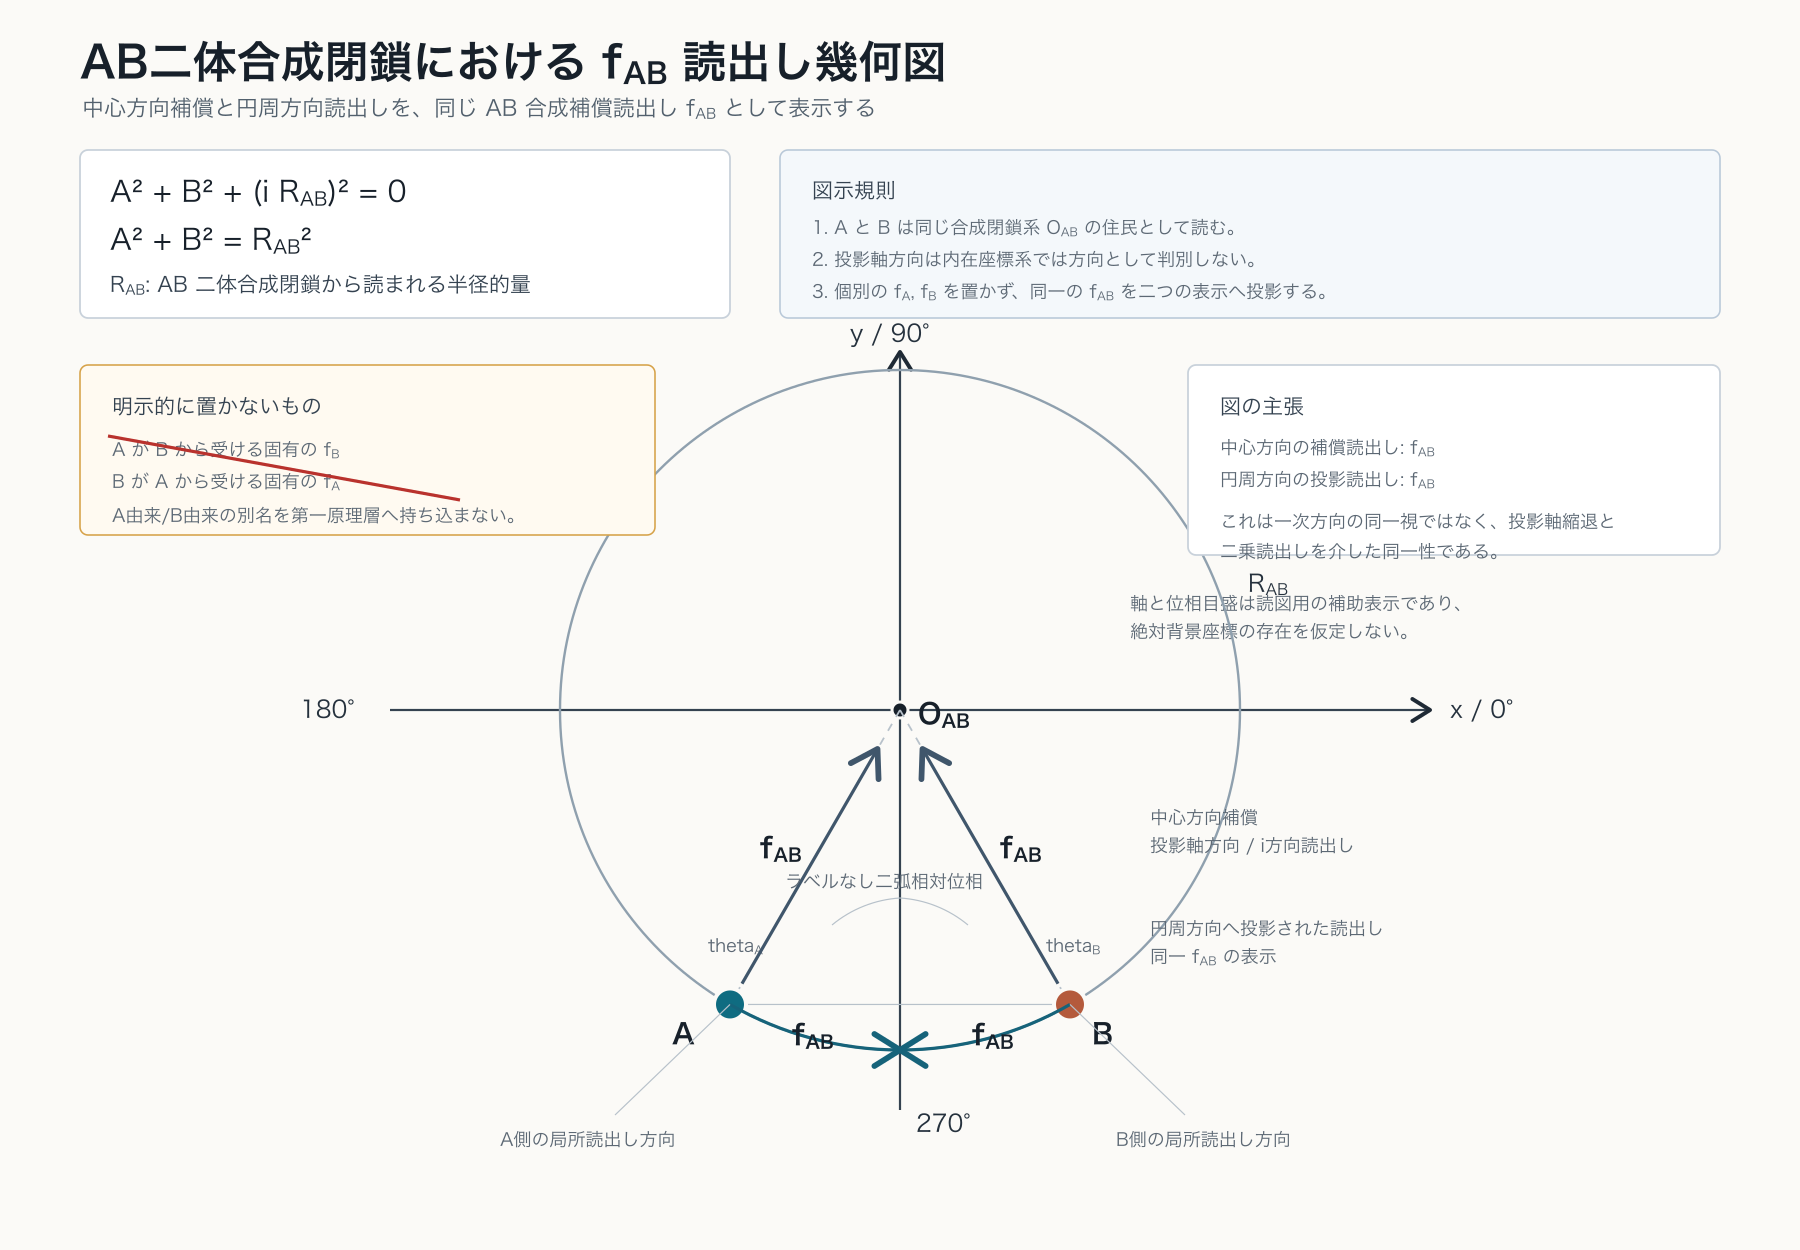
\includegraphics[keepaspectratio,alt={figure}]{AB二体問題の図化_fAB_v1.png}}
&
\pandocbounded{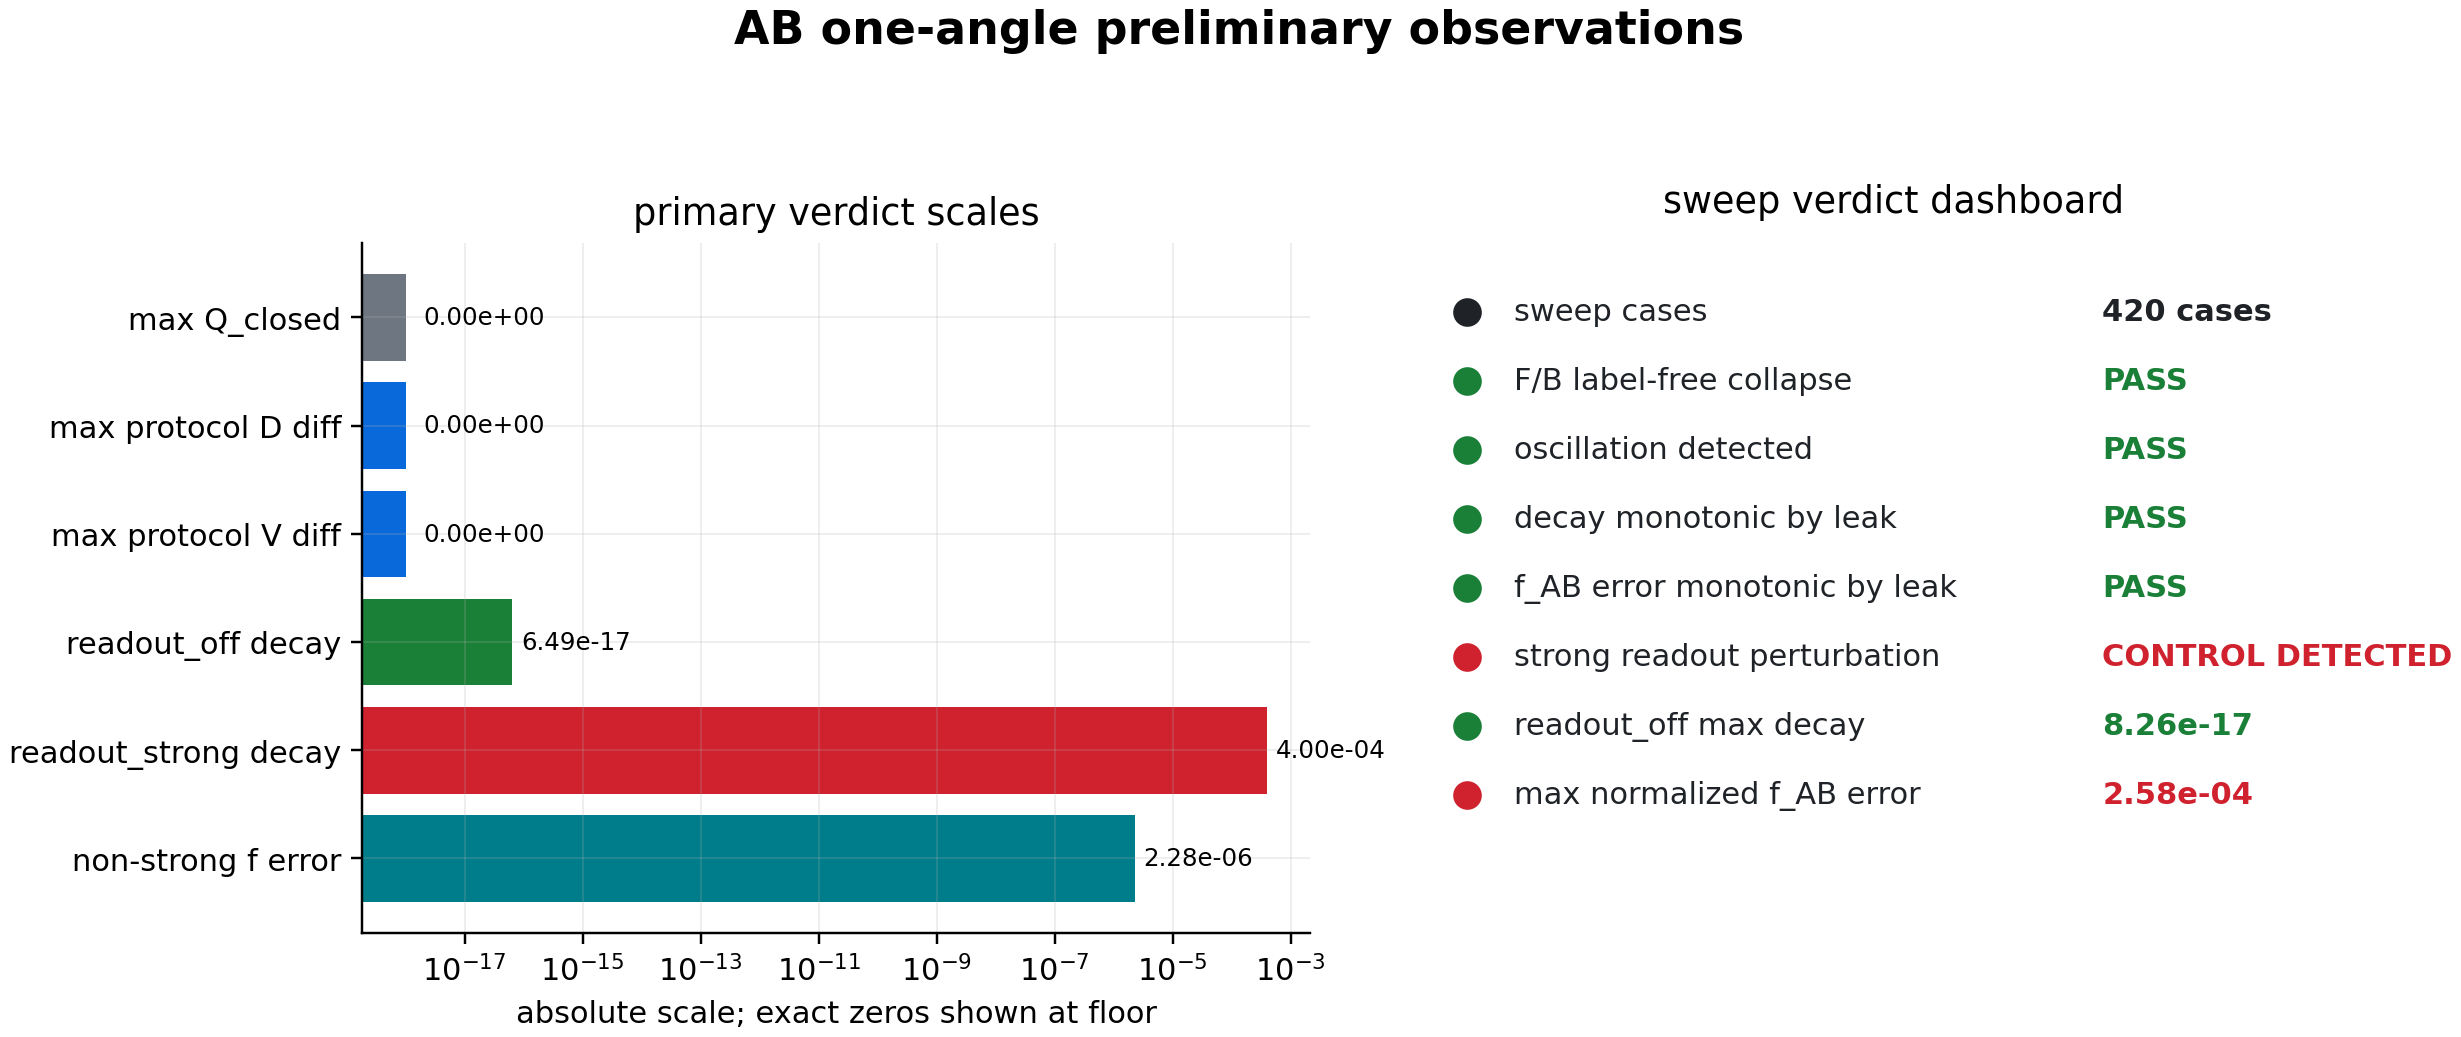
\includegraphics[keepaspectratio,alt={figure}]{ab_two_body_one_angle_harmonic_readout_observation_figures_v1/ab_two_body_one_angle_observation_summary_v1.png}} \\
\end{longtable}
}

{\def\LTcaptype{none} % do not increment counter
\begin{longtable}[]{@{}
  >{\raggedright\arraybackslash}p{(\linewidth - 2\tabcolsep) * \real{0.5000}}
  >{\raggedright\arraybackslash}p{(\linewidth - 2\tabcolsep) * \real{0.5000}}@{}}
\toprule\noalign{}
\begin{minipage}[b]{\linewidth}\raggedright
Harmonic state
\end{minipage} & \begin{minipage}[b]{\linewidth}\raggedright
Readout leak response
\end{minipage} \\
\midrule\noalign{}
\endhead
\bottomrule\noalign{}
\endlastfoot
\pandocbounded{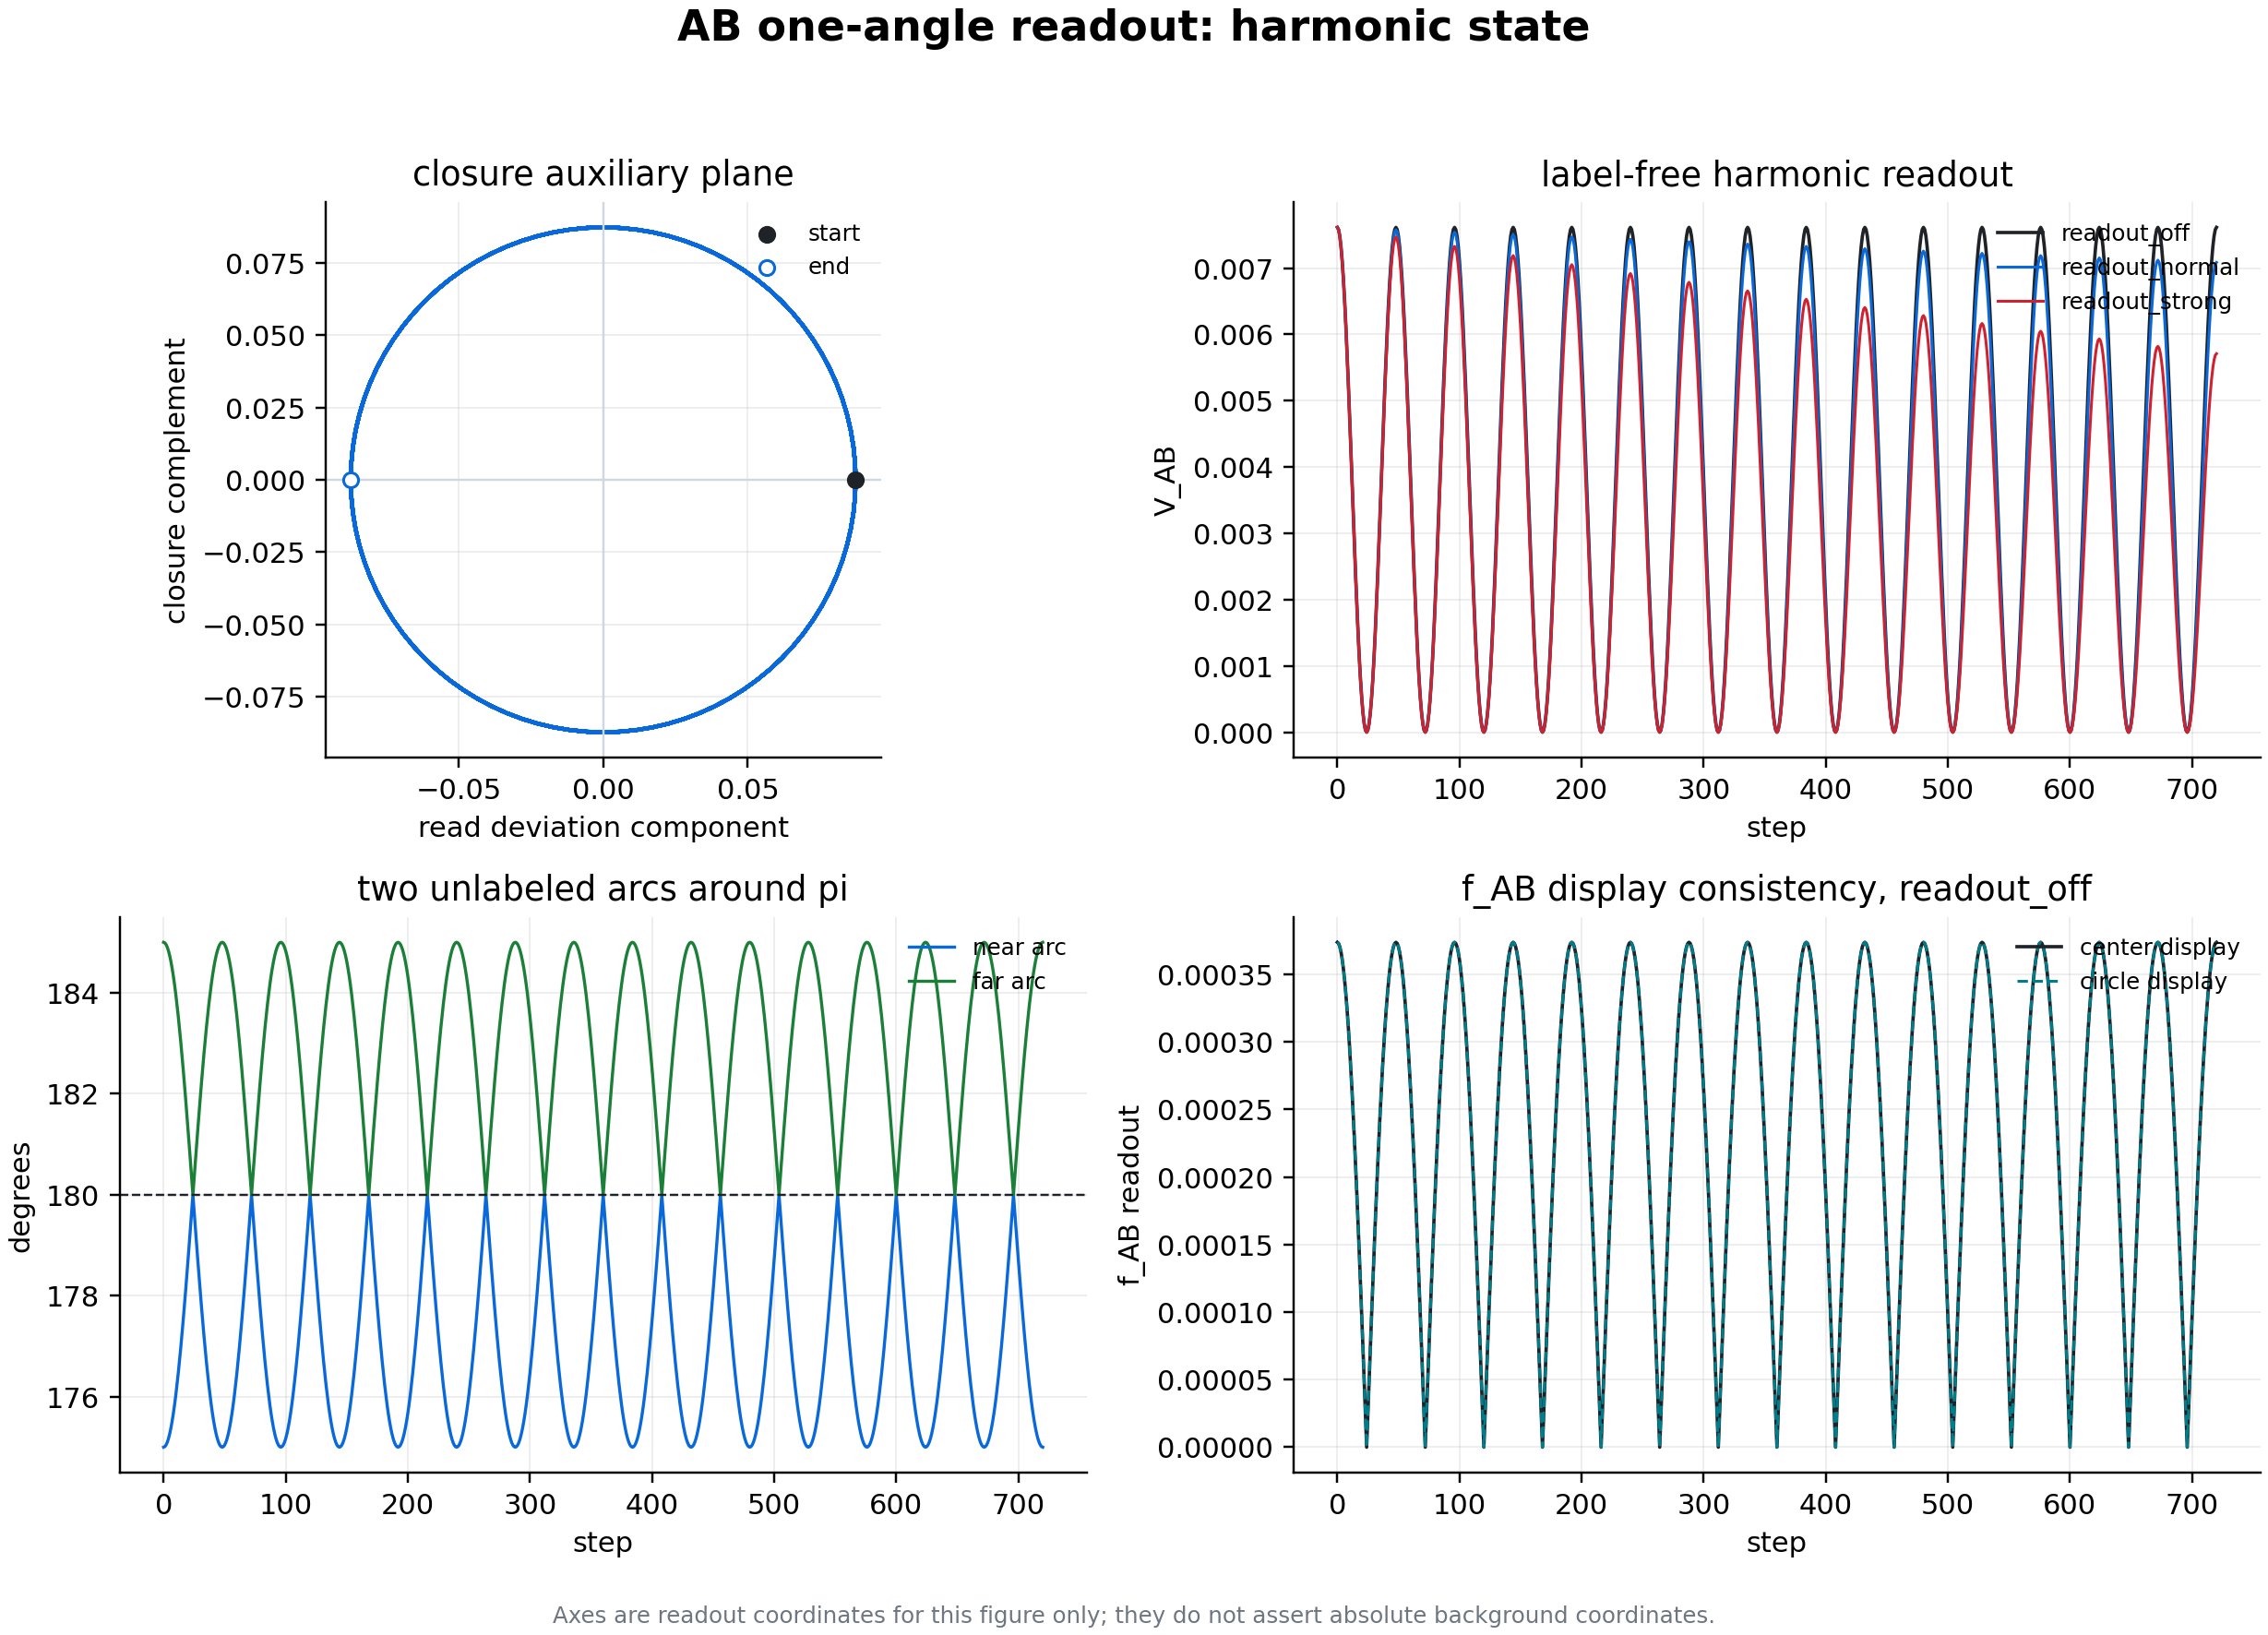
\includegraphics[keepaspectratio,alt={figure}]{ab_two_body_one_angle_harmonic_readout_observation_figures_v1/ab_two_body_one_angle_harmonic_state_v1.png}}
&
\pandocbounded{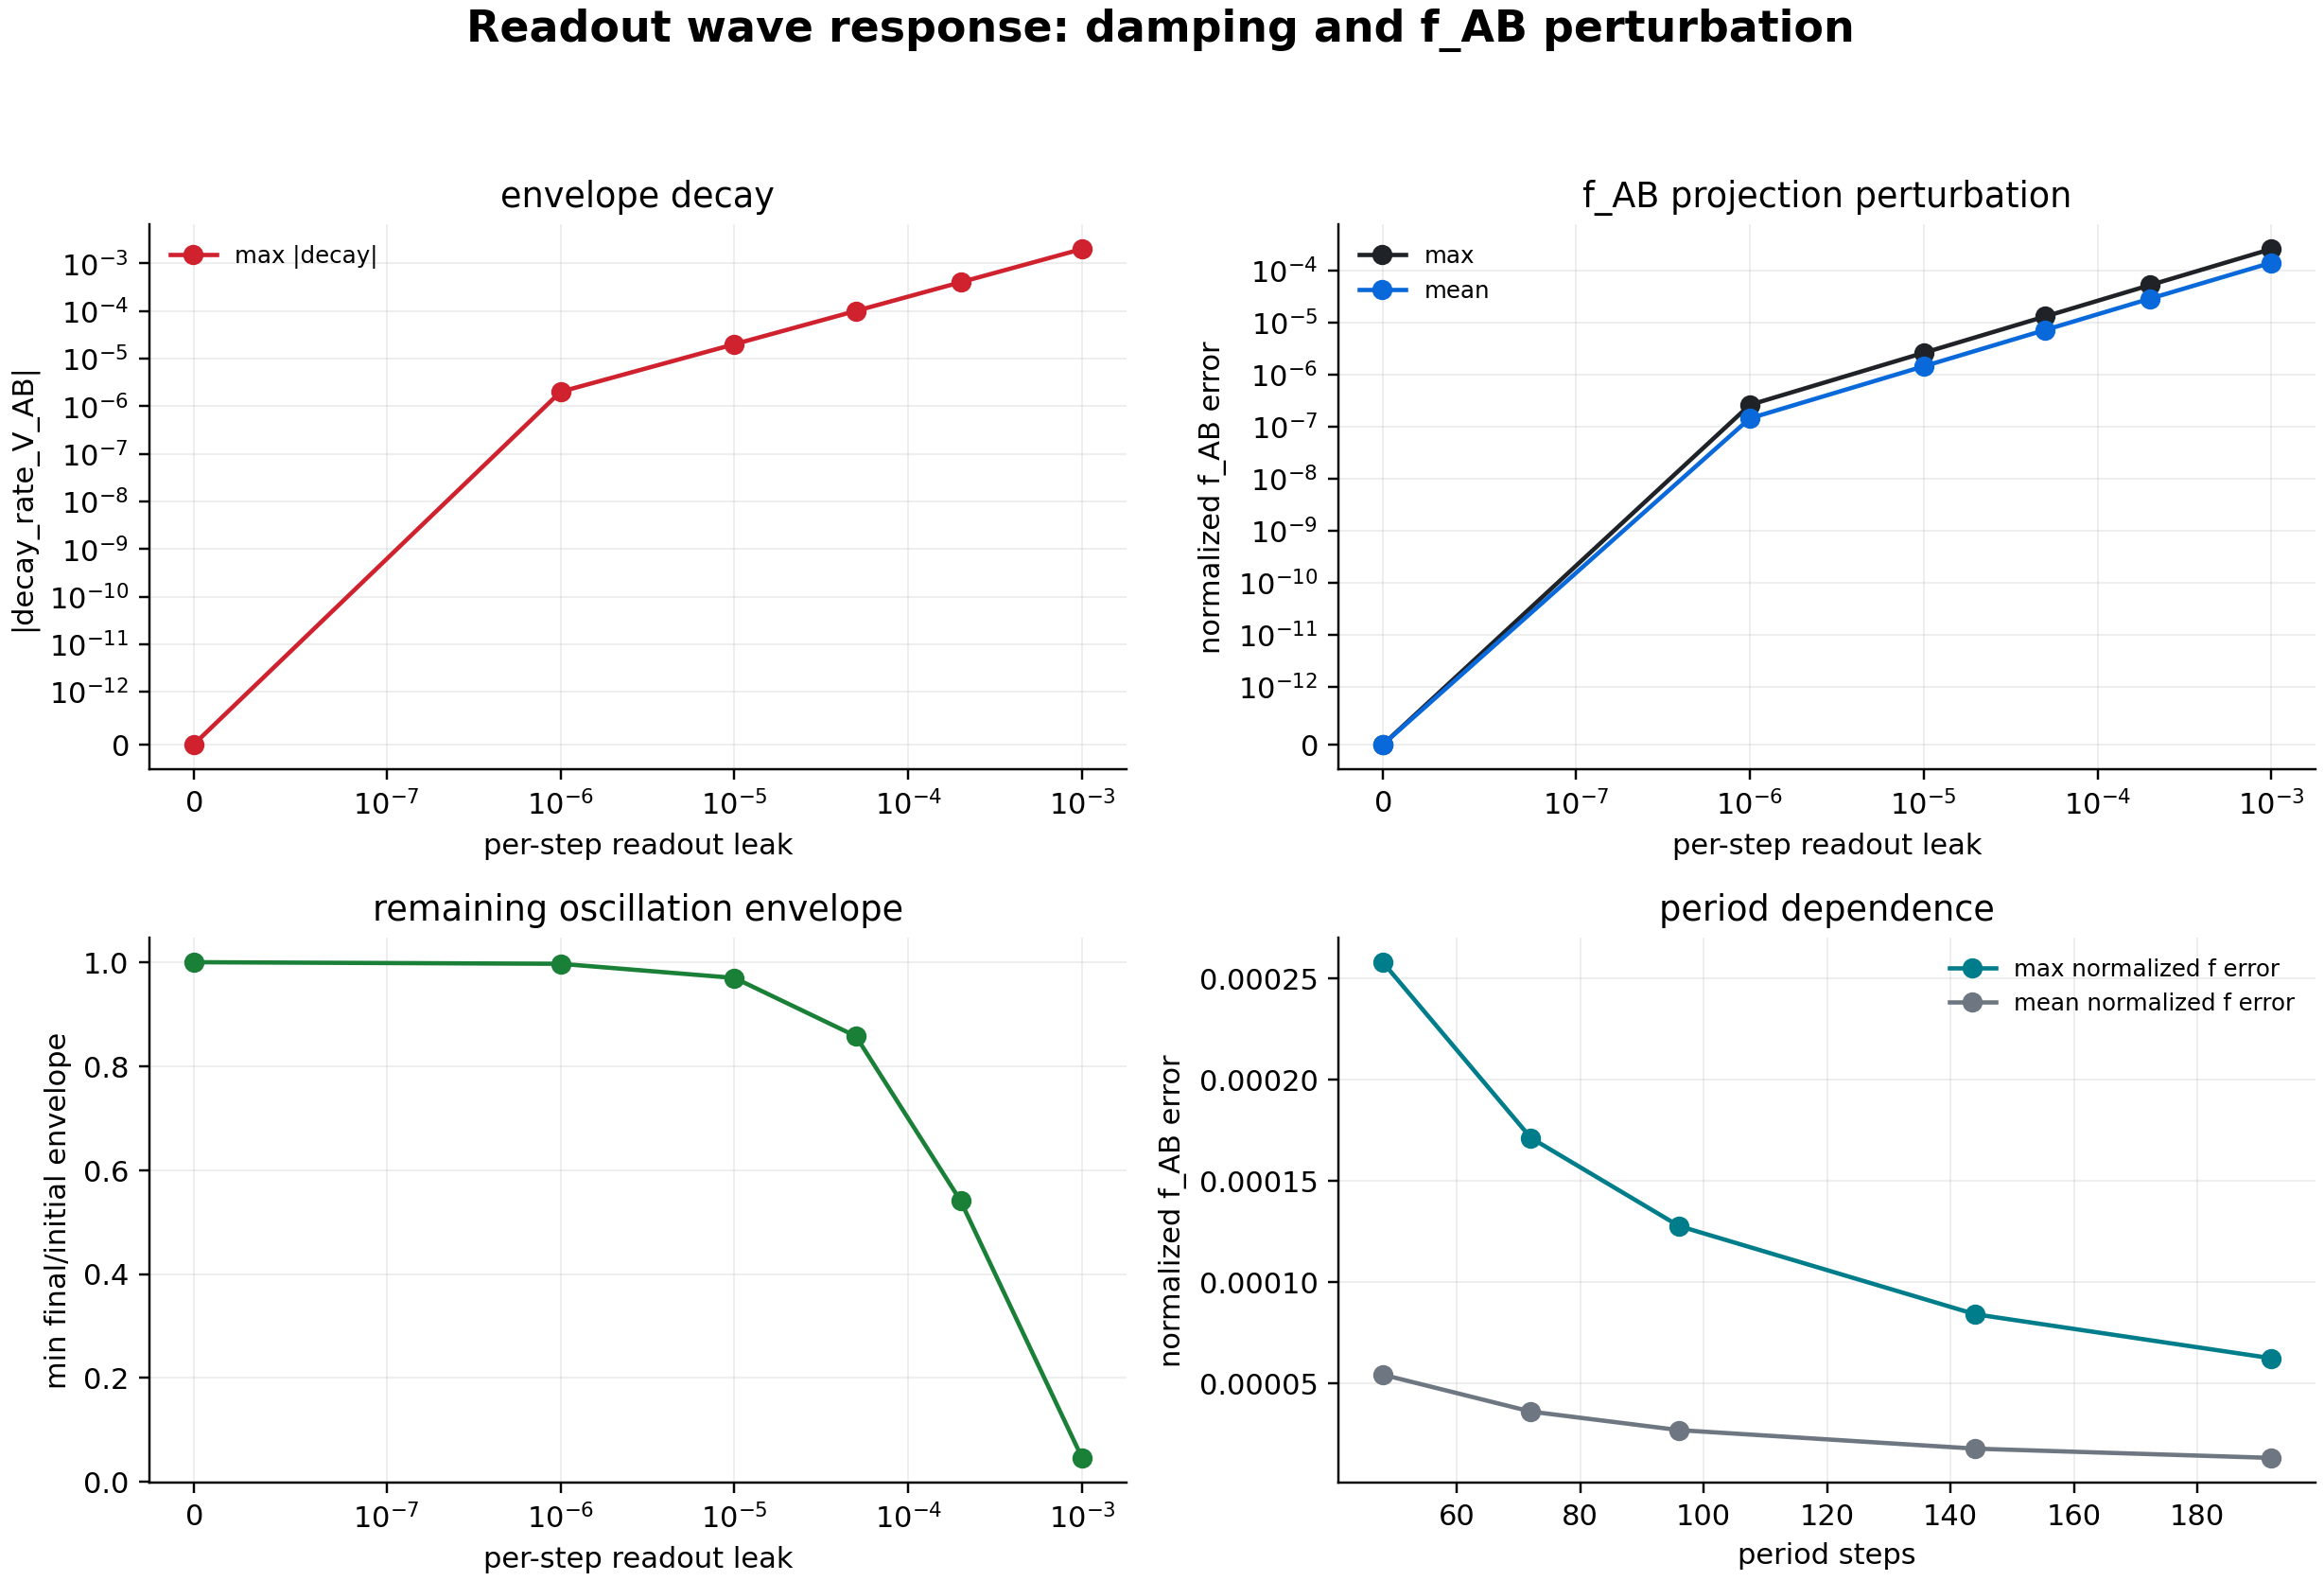
\includegraphics[keepaspectratio,alt={figure}]{ab_two_body_one_angle_harmonic_readout_observation_figures_v1/ab_two_body_one_angle_readout_leak_response_v1.png}} \\
\end{longtable}
}

{\def\LTcaptype{none} % do not increment counter
\begin{longtable}[]{@{}
  >{\raggedright\arraybackslash}p{(\linewidth - 2\tabcolsep) * \real{0.5000}}
  >{\raggedright\arraybackslash}p{(\linewidth - 2\tabcolsep) * \real{0.5000}}@{}}
\toprule\noalign{}
\begin{minipage}[b]{\linewidth}\raggedright
Protocol degeneracy
\end{minipage} & \begin{minipage}[b]{\linewidth}\raggedright
Phase-difference scaling
\end{minipage} \\
\midrule\noalign{}
\endhead
\bottomrule\noalign{}
\endlastfoot
\pandocbounded{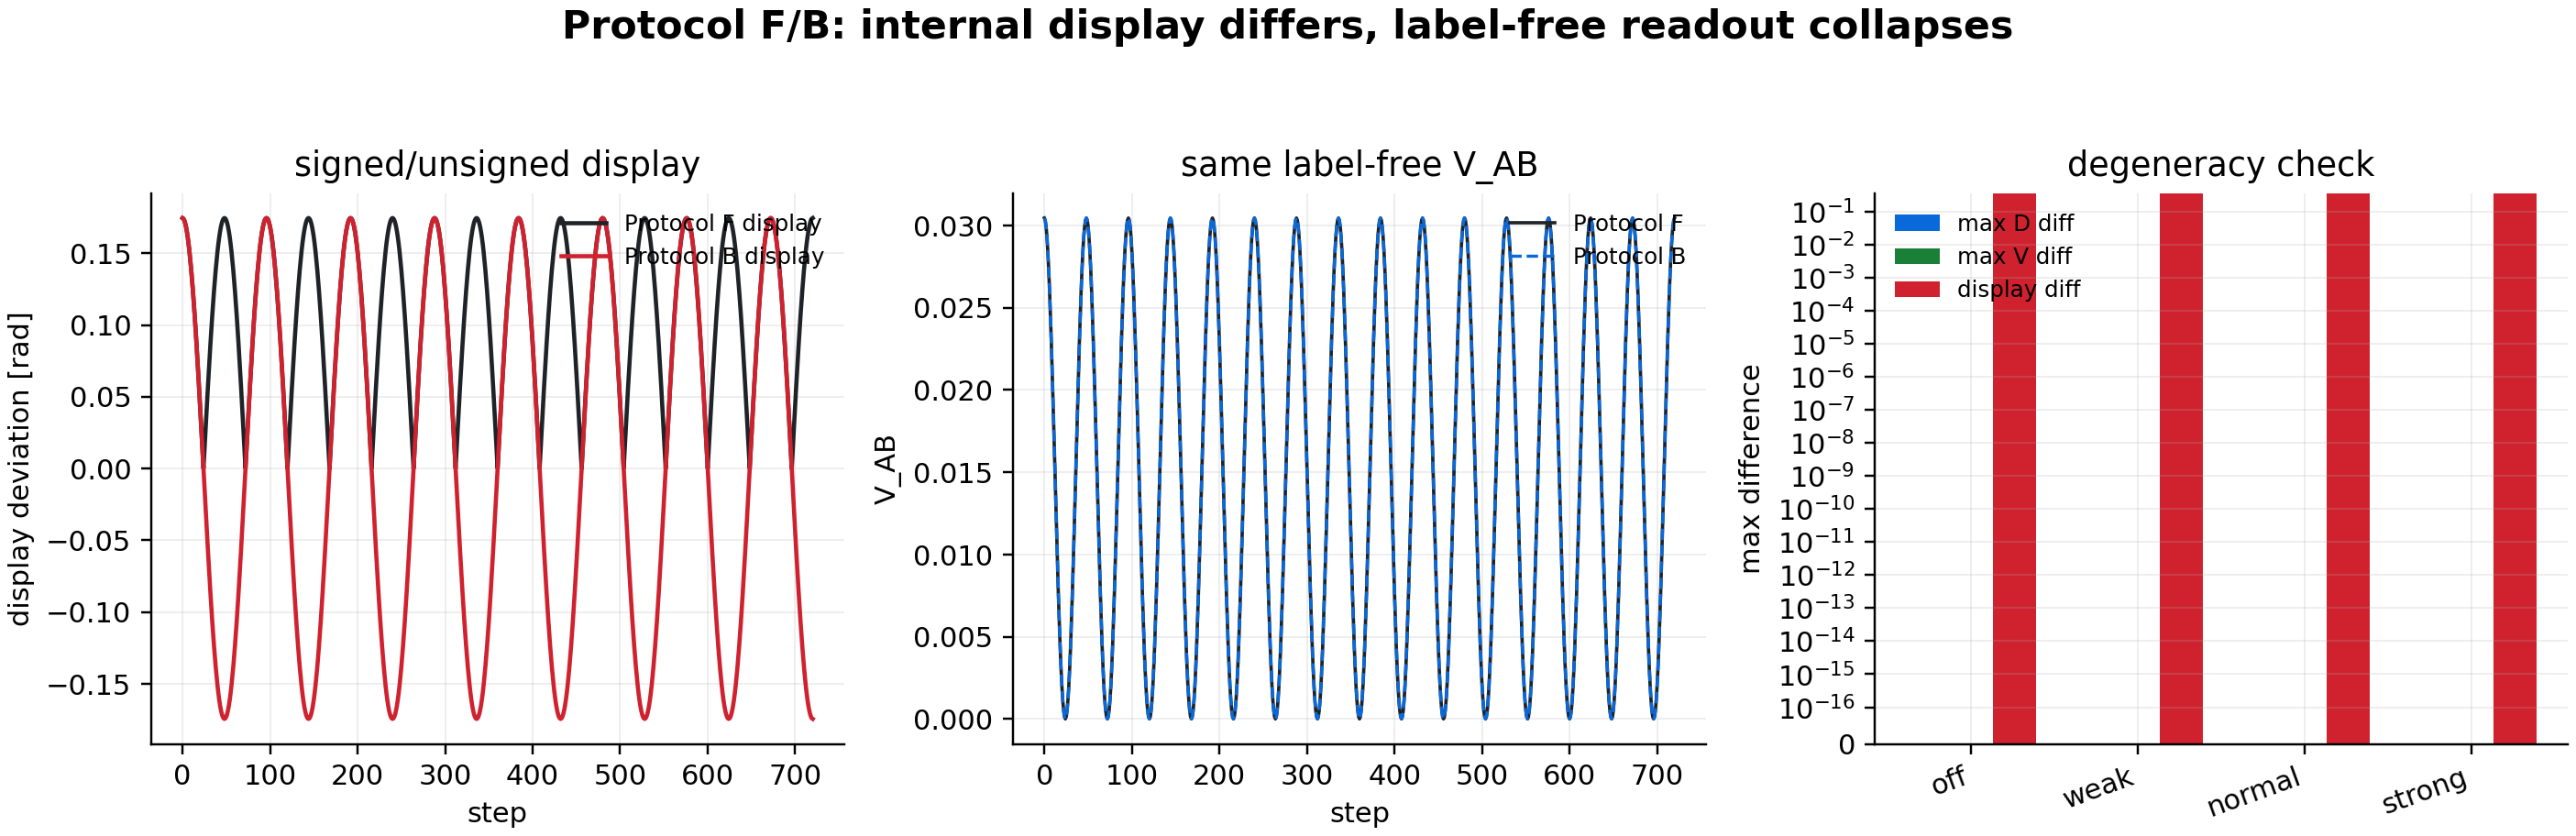
\includegraphics[keepaspectratio,alt={figure}]{ab_two_body_one_angle_harmonic_readout_observation_figures_v1/ab_two_body_one_angle_protocol_degeneracy_v1.png}}
&
\pandocbounded{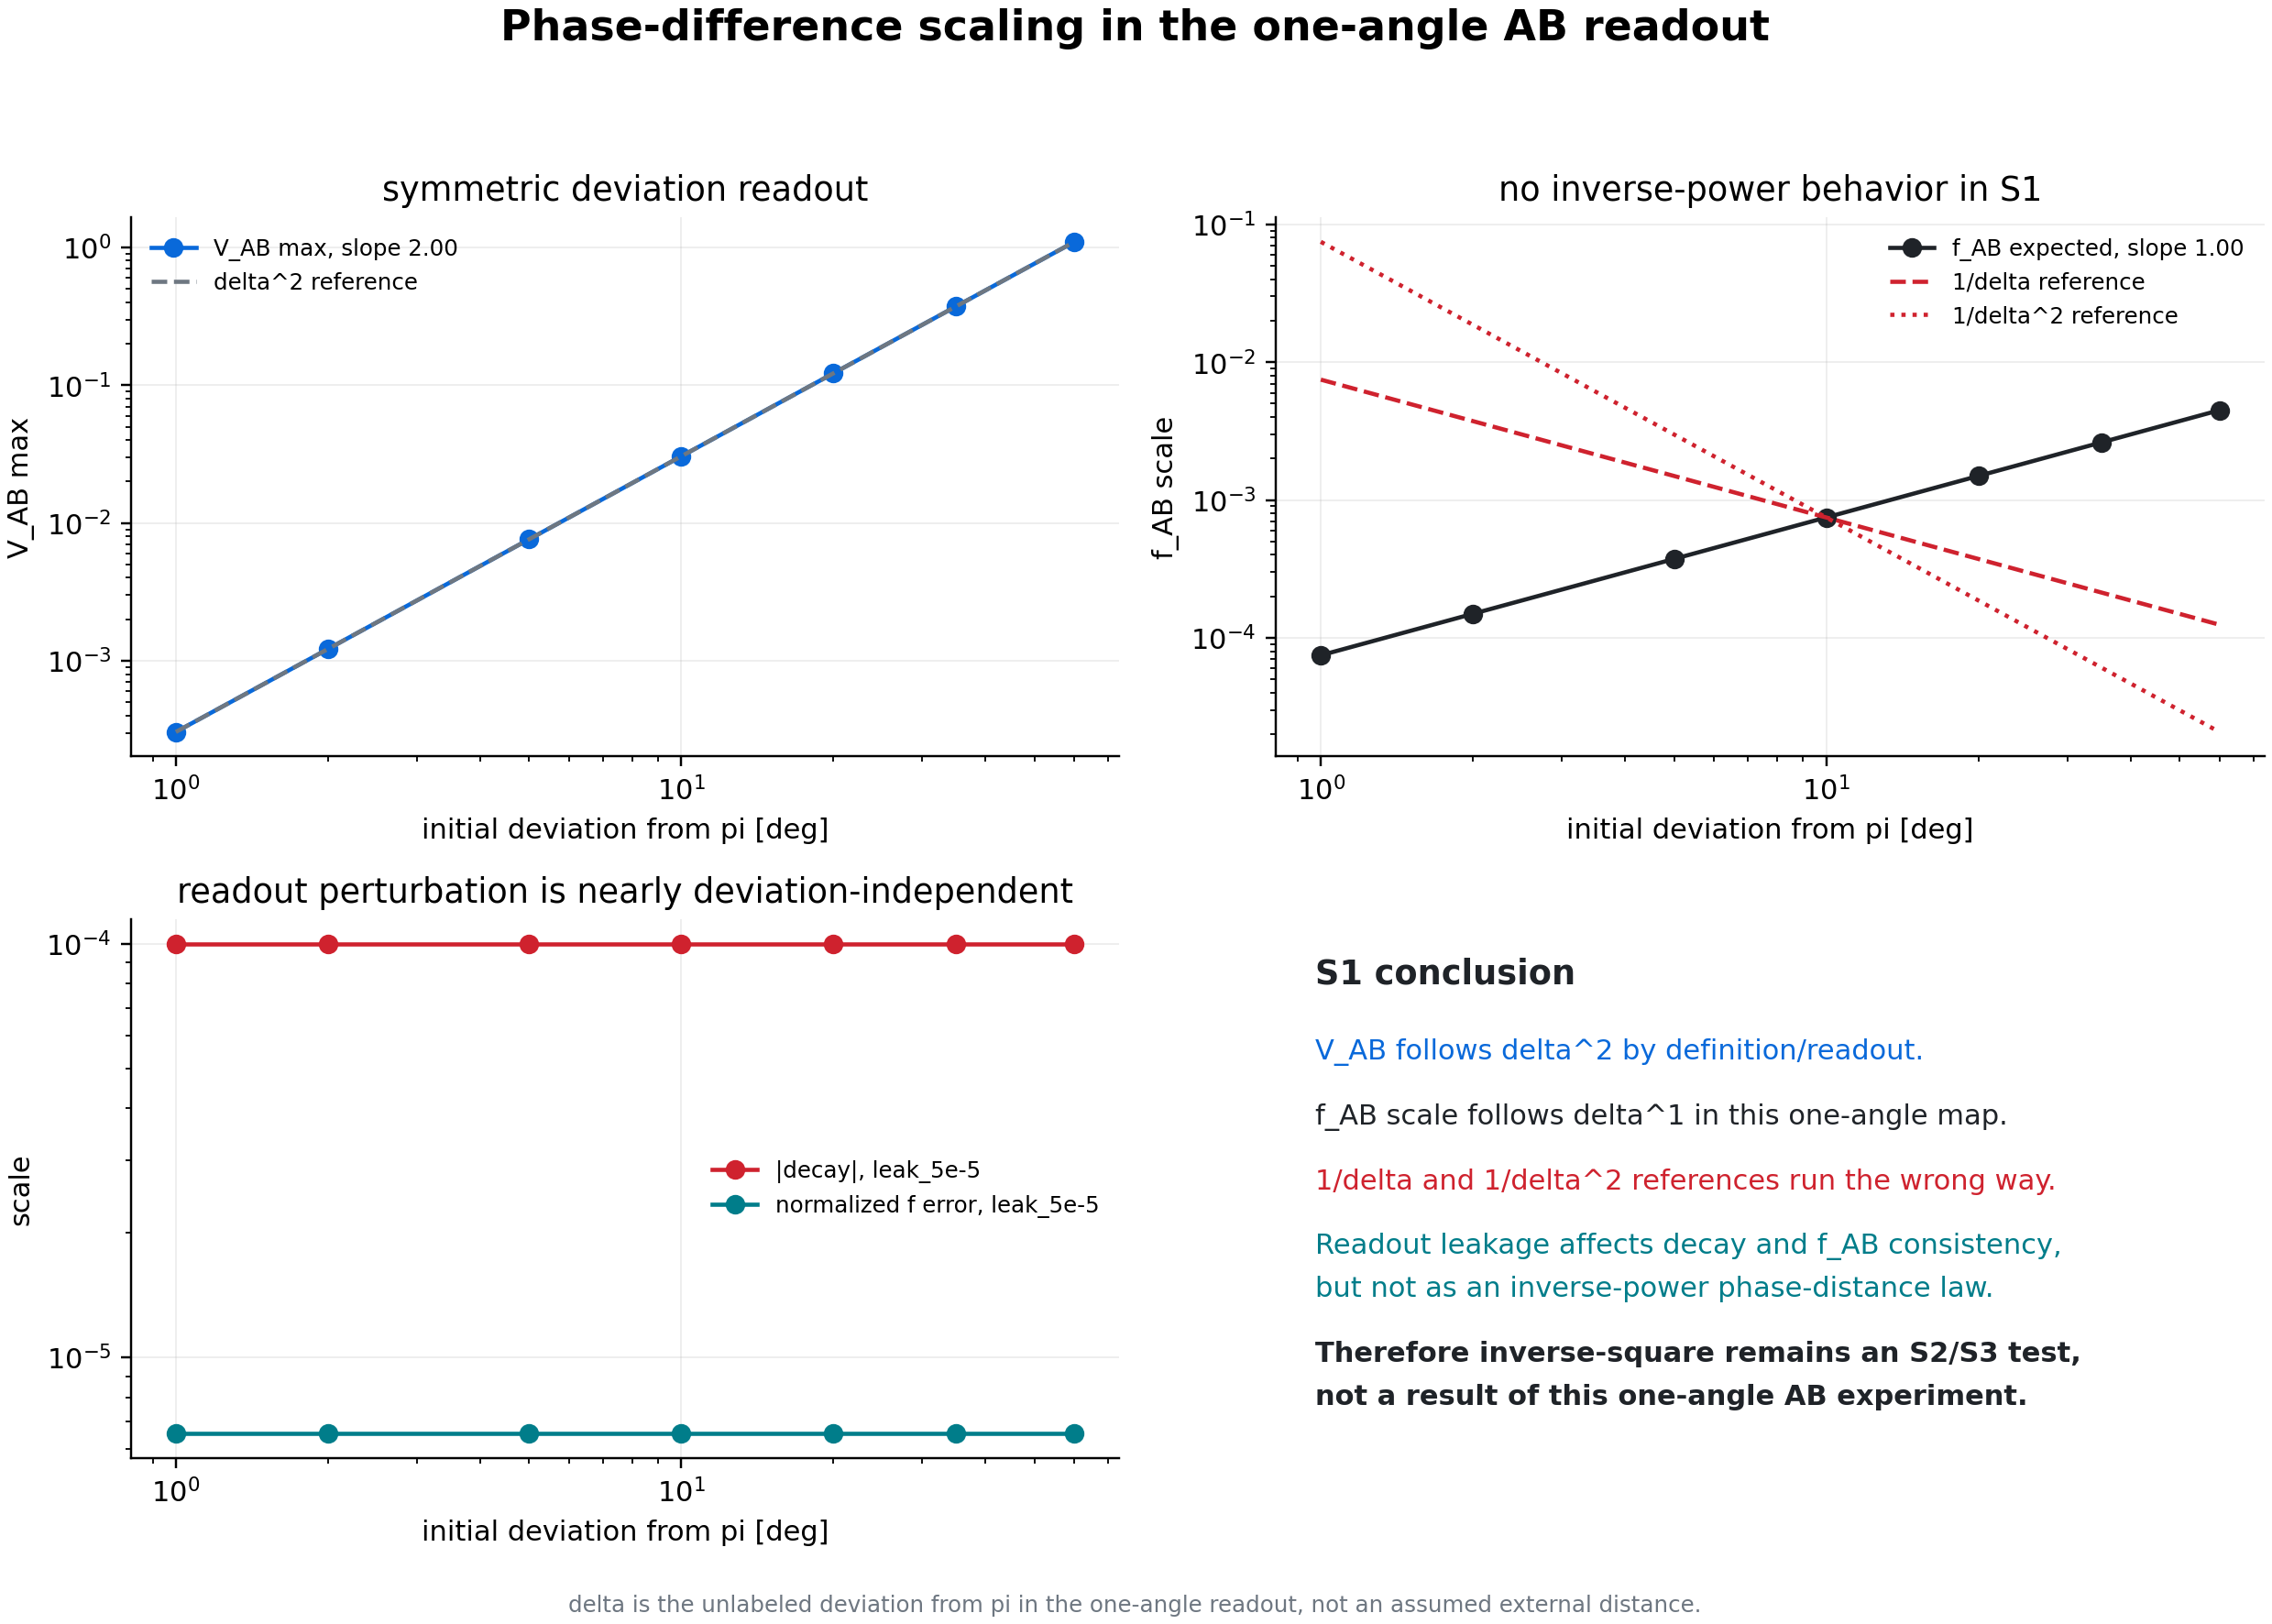
\includegraphics[keepaspectratio,alt={figure}]{ab_two_body_one_angle_harmonic_readout_observation_figures_v1/ab_two_body_one_angle_phase_difference_scaling_v1.png}} \\
\end{longtable}
}

\begin{center}\rule{0.5\linewidth}{0.5pt}\end{center}

\subsection{3. One-Angle Parameter
Sweep}\label{one-angle-parameter-sweep}

\subsubsection{3.1 Main Result}\label{main-result-1}

{\def\LTcaptype{none} % do not increment counter
\begin{longtable}[]{@{}lr@{}}
\toprule\noalign{}
Quantity & Value \\
\midrule\noalign{}
\endhead
\bottomrule\noalign{}
\endlastfoot
\texttt{sweep\_configuration\_count} & \texttt{210} \\
\texttt{case\_summary\_count} & \texttt{420} \\
\texttt{period\_count} & \texttt{5} \\
\texttt{deviation\_count} & \texttt{7} \\
\texttt{leak\_count} & \texttt{6} \\
\texttt{max\_Q\_closed\_abs} & \texttt{0.0} \\
\texttt{label\_free\_protocol\_degenerate\_all\_cases} &
\texttt{True} \\
\texttt{oscillation\_detected\_all\_cases} & \texttt{True} \\
\texttt{readout\_off\_decay\_max\_abs} & \texttt{8.26e-17} \\
\texttt{decay\_abs\_monotonic\_by\_leak\_all\_grids} & \texttt{True} \\
\texttt{max\_normalized\_f\_AB\_projection\_error} & \texttt{2.58e-4} \\
\end{longtable}
}

This sweep confirmed that the one-angle version is stable under weak
readout, while a strong readout wave distorts the \texttt{f\_AB}
projection.

{\def\LTcaptype{none} % do not increment counter
\begin{longtable}[]{@{}
  >{\raggedright\arraybackslash}p{(\linewidth - 2\tabcolsep) * \real{0.5000}}
  >{\raggedright\arraybackslash}p{(\linewidth - 2\tabcolsep) * \real{0.5000}}@{}}
\toprule\noalign{}
\begin{minipage}[b]{\linewidth}\raggedright
Leakage and projection error
\end{minipage} & \begin{minipage}[b]{\linewidth}\raggedright
Leakage and decay
\end{minipage} \\
\midrule\noalign{}
\endhead
\bottomrule\noalign{}
\endlastfoot
\pandocbounded{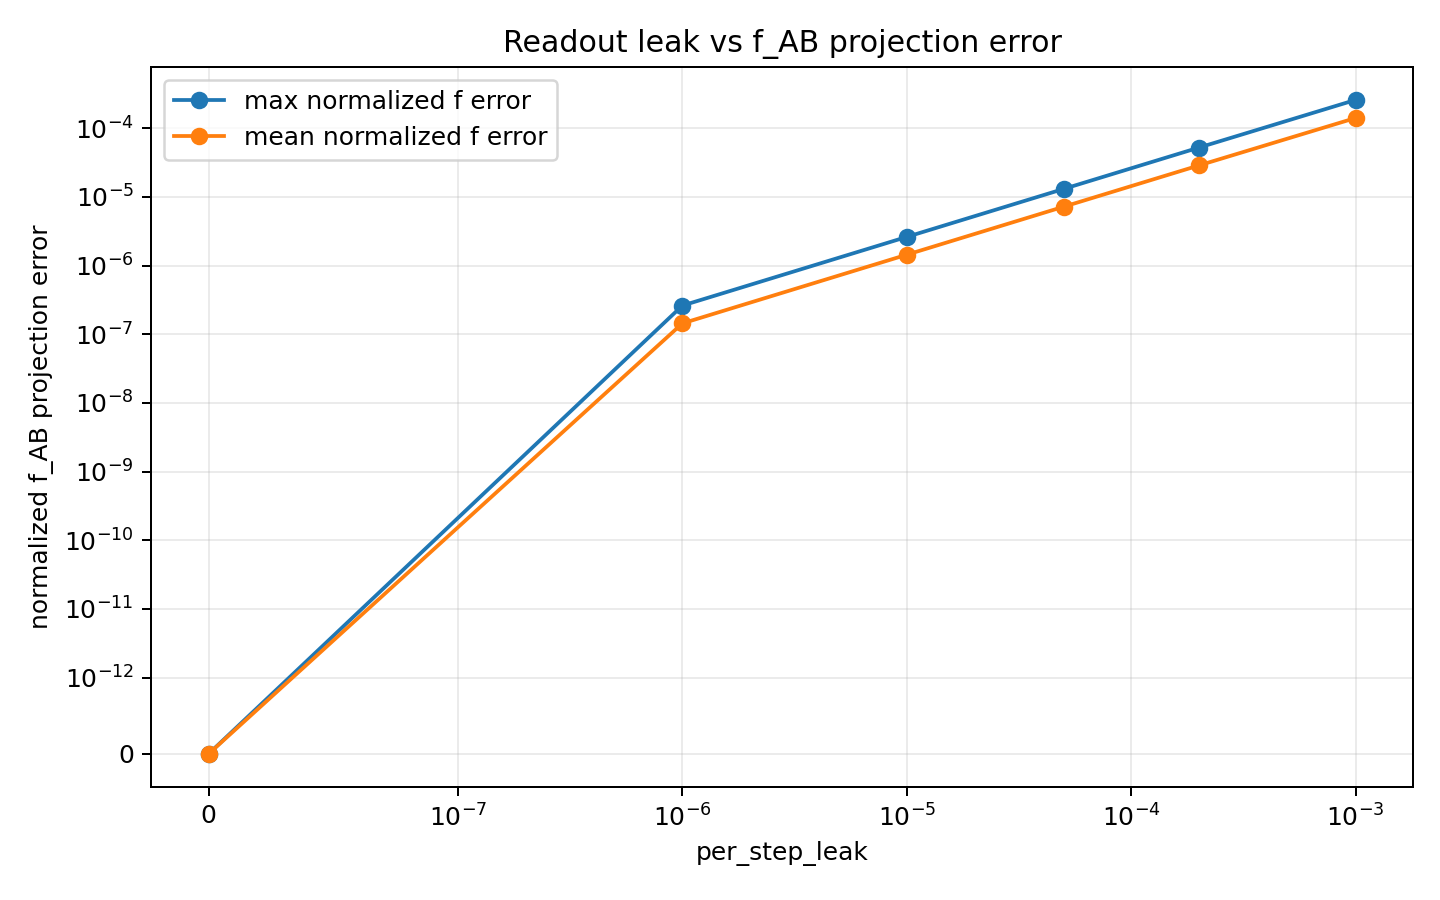
\includegraphics[keepaspectratio,alt={figure}]{ab_two_body_one_angle_harmonic_readout_parameter_sweep_preliminary_result_v1/ab_two_body_one_angle_parameter_sweep_leak_f_error_v1.png}}
&
\pandocbounded{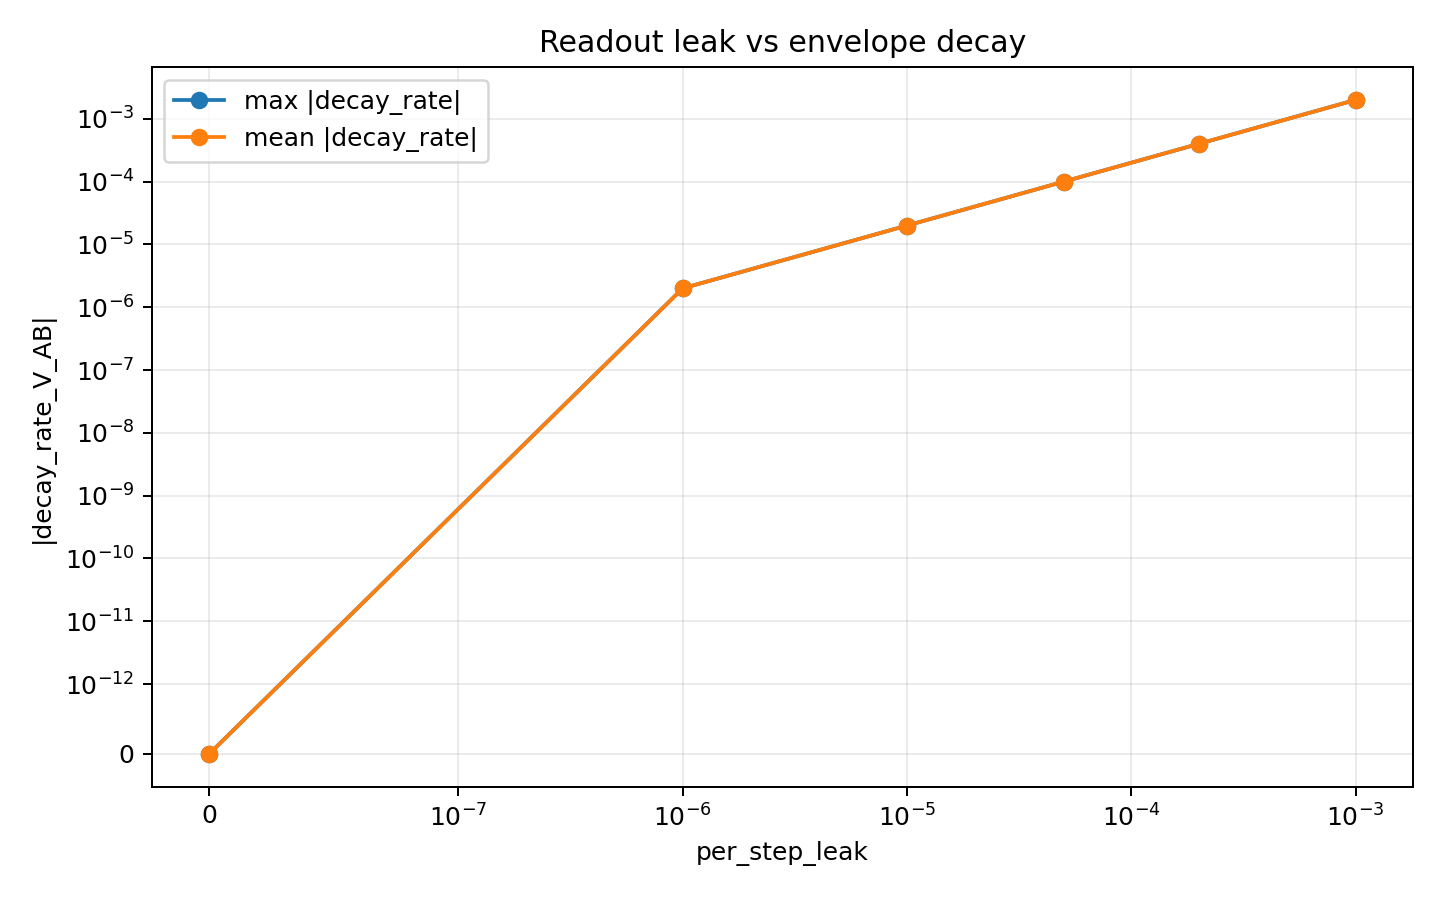
\includegraphics[keepaspectratio,alt={figure}]{ab_two_body_one_angle_harmonic_readout_parameter_sweep_preliminary_result_v1/ab_two_body_one_angle_parameter_sweep_leak_decay_v1.png}} \\
\end{longtable}
}

{\def\LTcaptype{none} % do not increment counter
\begin{longtable}[]{@{}
  >{\raggedright\arraybackslash}p{(\linewidth - 2\tabcolsep) * \real{0.5000}}
  >{\raggedright\arraybackslash}p{(\linewidth - 2\tabcolsep) * \real{0.5000}}@{}}
\toprule\noalign{}
\begin{minipage}[b]{\linewidth}\raggedright
Period sweep
\end{minipage} & \begin{minipage}[b]{\linewidth}\raggedright
Selected time series
\end{minipage} \\
\midrule\noalign{}
\endhead
\bottomrule\noalign{}
\endlastfoot
\pandocbounded{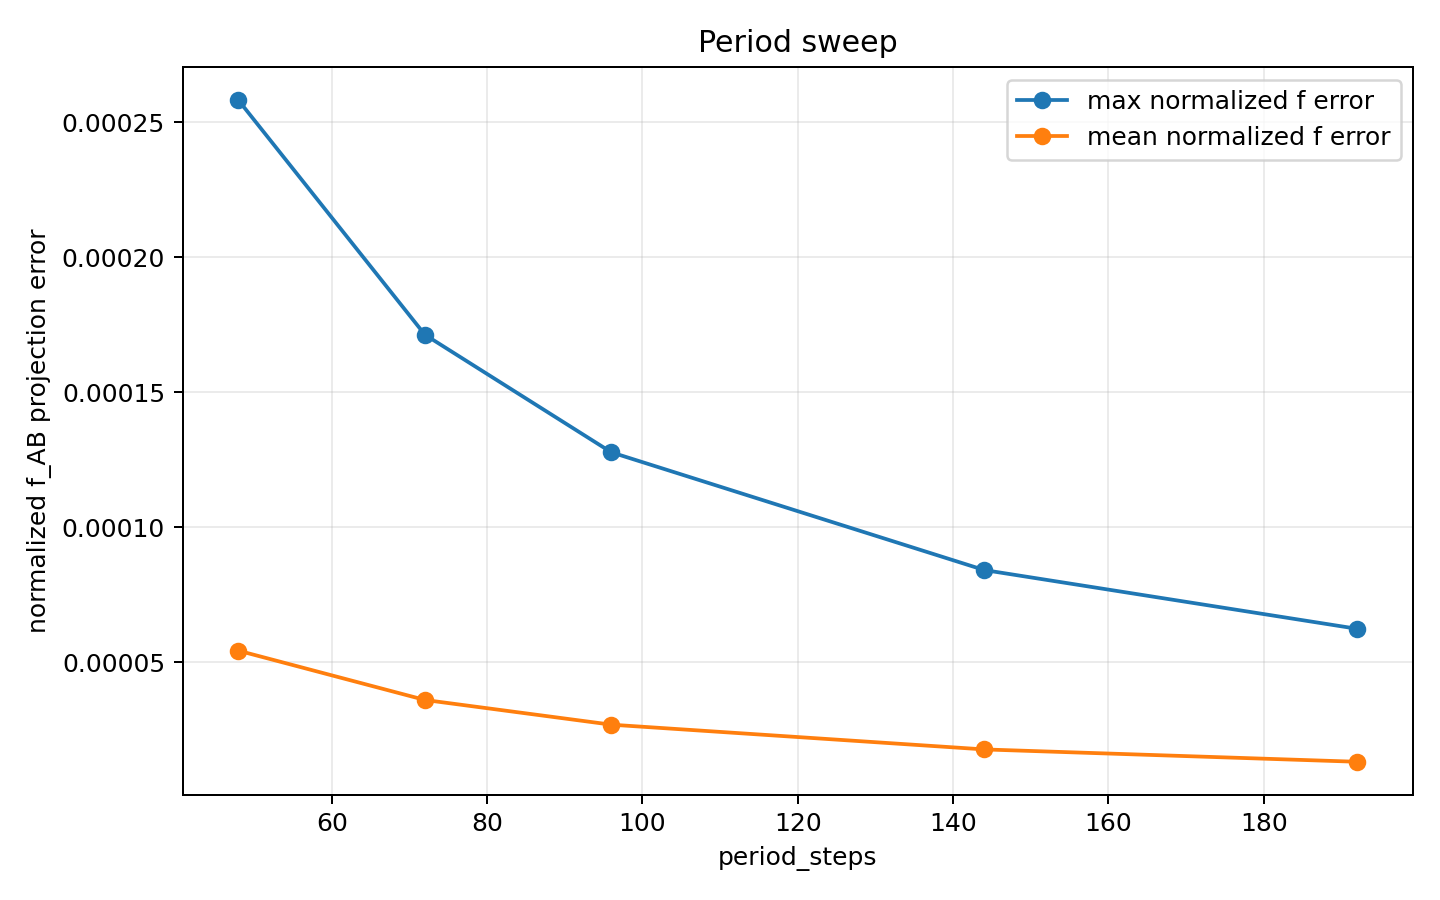
\includegraphics[keepaspectratio,alt={figure}]{ab_two_body_one_angle_harmonic_readout_parameter_sweep_preliminary_result_v1/ab_two_body_one_angle_parameter_sweep_period_v1.png}}
&
\pandocbounded{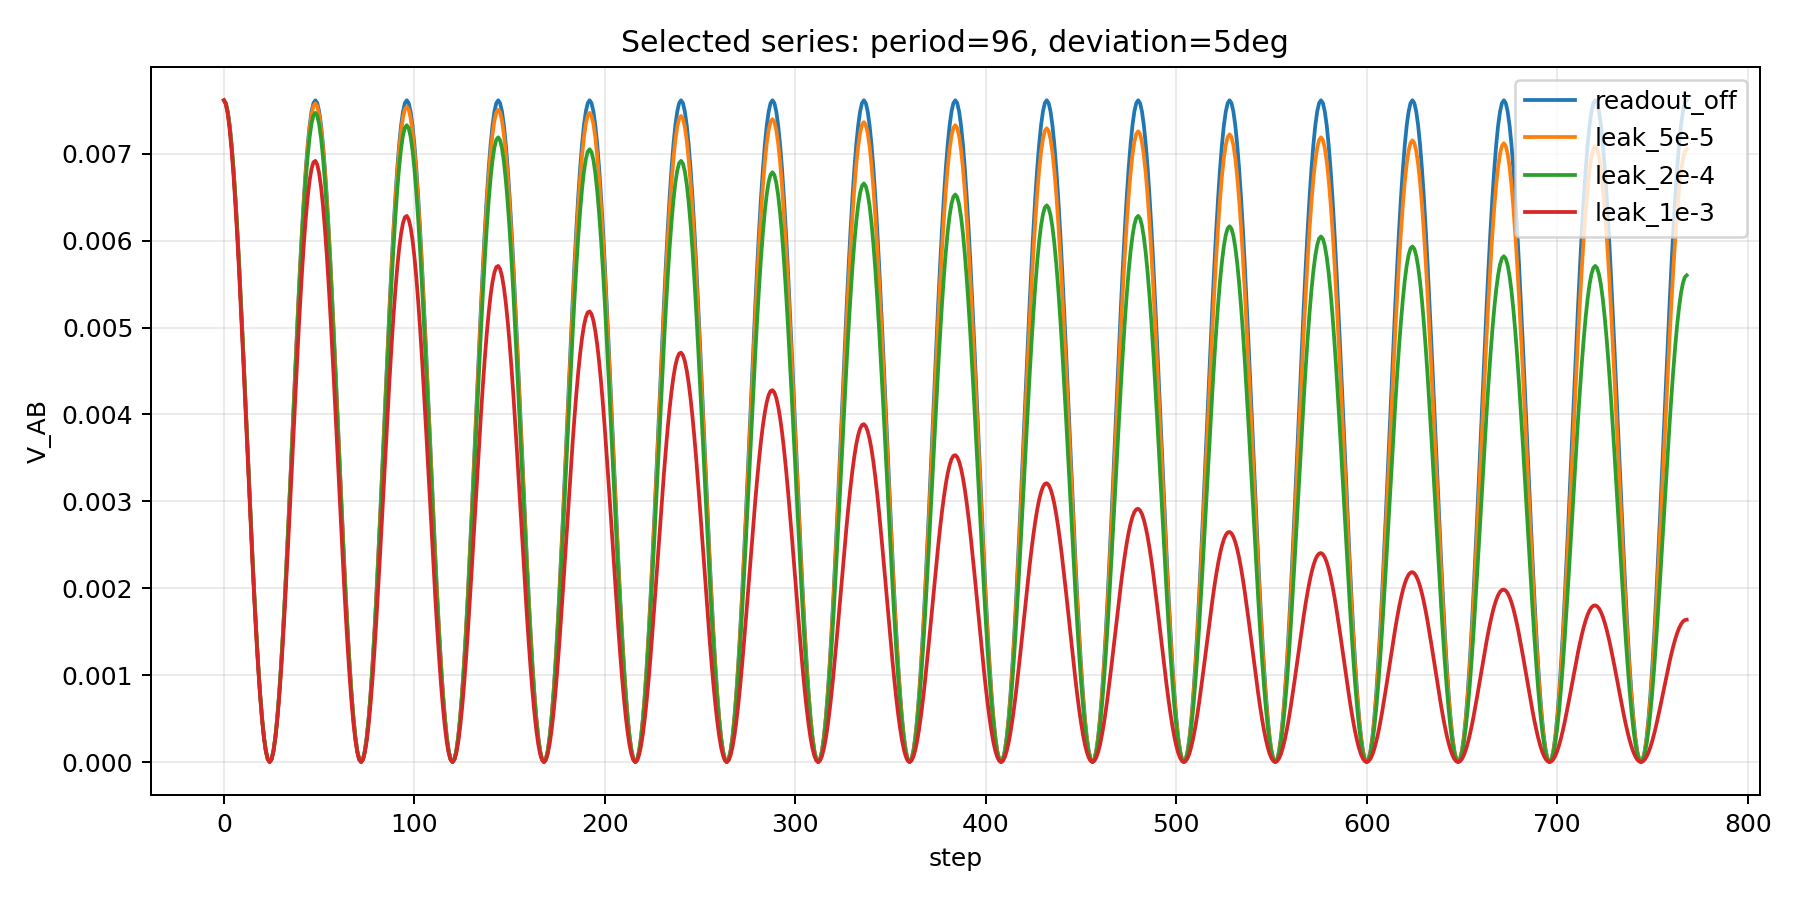
\includegraphics[keepaspectratio,alt={figure}]{ab_two_body_one_angle_harmonic_readout_parameter_sweep_preliminary_result_v1/ab_two_body_one_angle_parameter_sweep_selected_series_v1.png}} \\
\end{longtable}
}

\begin{center}\rule{0.5\linewidth}{0.5pt}\end{center}

\subsection{4. c=1 Internal Calibration and chi-tau Area
Sweep}\label{c1-internal-calibration-and-chi-tau-area-sweep}

\subsubsection{4.1 Meaning of the
Experiment}\label{meaning-of-the-experiment-1}

In the one-angle harmonic readout, distance attenuation according to
phase difference was not read.

Therefore, the experiment step \texttt{s} was not treated as time
itself. Instead, an independent temporal phase candidate

\begin{Shaded}
\begin{Highlighting}[]
\NormalTok{tau\_read}
\end{Highlighting}
\end{Shaded}

was introduced.

The purpose was to test whether

\begin{Shaded}
\begin{Highlighting}[]
\NormalTok{chi\_read and tau\_read form an independent plane.}
\end{Highlighting}
\end{Shaded}

\subsubsection{4.2 Main Result}\label{main-result-2}

{\def\LTcaptype{none} % do not increment counter
\begin{longtable}[]{@{}lr@{}}
\toprule\noalign{}
Quantity & Value \\
\midrule\noalign{}
\endhead
\bottomrule\noalign{}
\endlastfoot
\texttt{case\_summary\_count} & \texttt{288} \\
\texttt{power\_candidate\_count} & \texttt{48} \\
\texttt{max\_Q\_closed\_abs} & \texttt{0.0} \\
\texttt{disabled\_max\_area} & \texttt{0.0} \\
\texttt{locked\_max\_area} & \texttt{7.11e-15} \\
\texttt{independent\_min\_area} & \texttt{0.0024367633602631385} \\
\texttt{c1\_readout\_off\_max\_epsilon\_c\_abs} & \texttt{2.33e-15} \\
\texttt{c1\_area\_sweep\_detected\_all\_cases} & \texttt{True} \\
\texttt{tau\_is\_step\_used\_any} & \texttt{False} \\
\texttt{external\_c\_used\_any} & \texttt{False} \\
\end{longtable}
}

The following was established.

\begin{Shaded}
\begin{Highlighting}[]
\NormalTok{tau disabled does not create area.}
\NormalTok{tau locked does not create area.}
\NormalTok{tau independent creates chi{-}tau area.}
\end{Highlighting}
\end{Shaded}

Thus, an independent temporal phase can make the \texttt{chi-tau} plane
stand.

However, this alone does not generate distance attenuation.

\subsubsection{4.3 Figures}\label{figures-1}

{\def\LTcaptype{none} % do not increment counter
\begin{longtable}[]{@{}
  >{\raggedright\arraybackslash}p{(\linewidth - 2\tabcolsep) * \real{0.5000}}
  >{\raggedright\arraybackslash}p{(\linewidth - 2\tabcolsep) * \real{0.5000}}@{}}
\toprule\noalign{}
\begin{minipage}[b]{\linewidth}\raggedright
\texttt{chi-tau} surface
\end{minipage} & \begin{minipage}[b]{\linewidth}\raggedright
Area sweep
\end{minipage} \\
\midrule\noalign{}
\endhead
\bottomrule\noalign{}
\endlastfoot
\pandocbounded{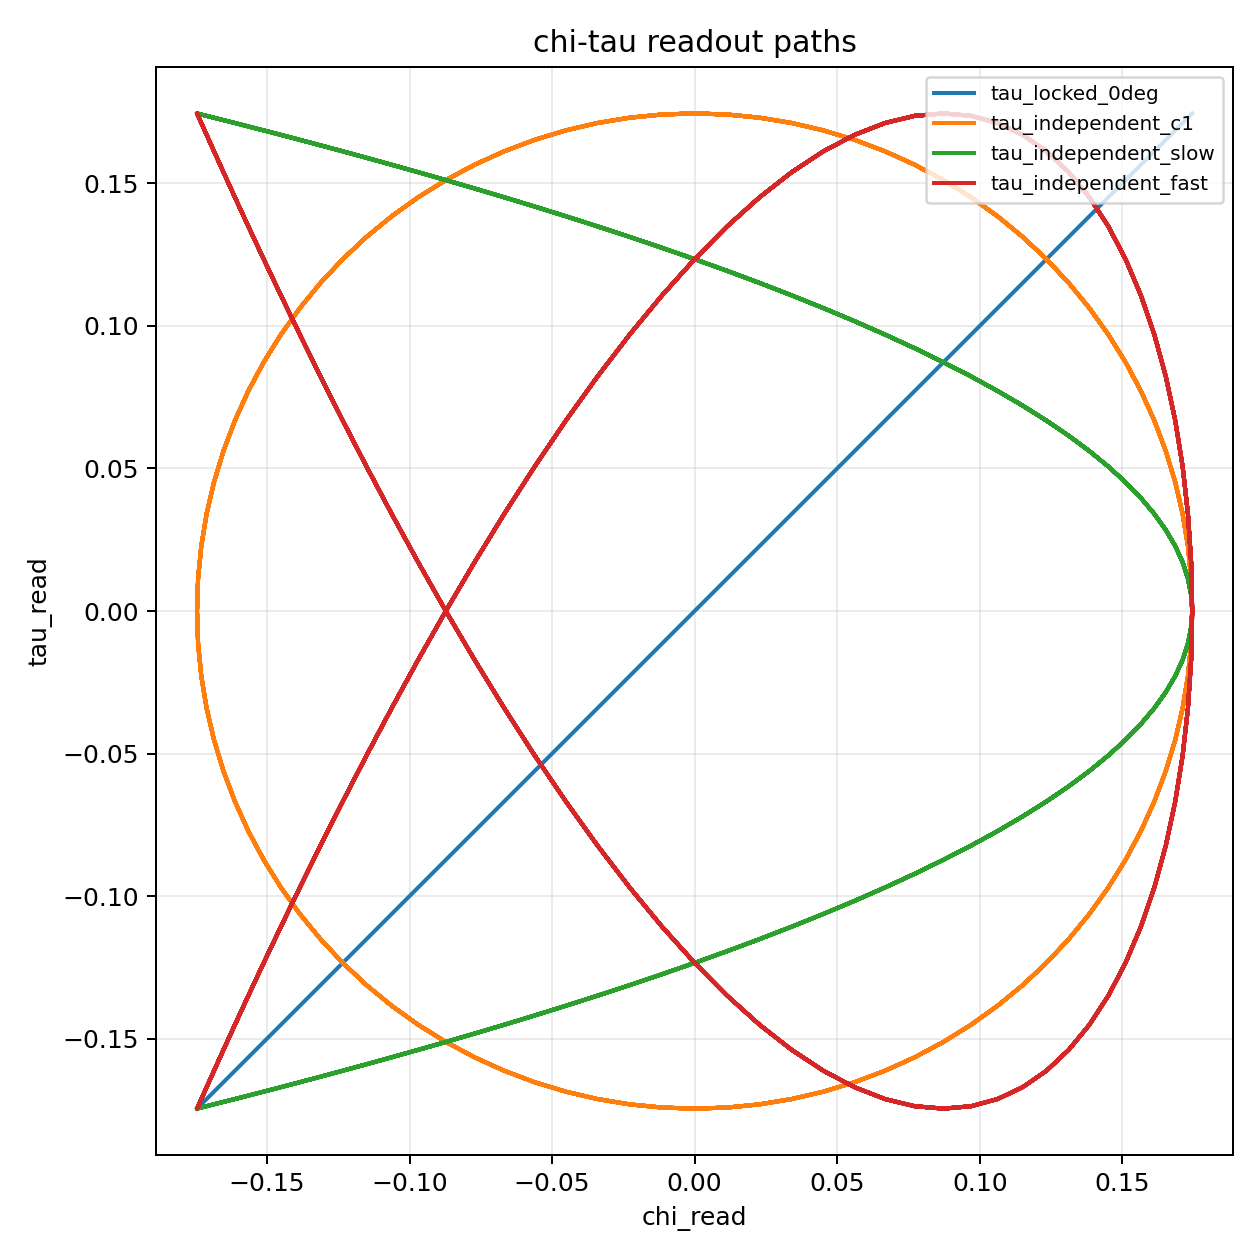
\includegraphics[keepaspectratio,alt={figure}]{ab_two_body_c1_internal_calibration_chi_tau_area_sweep_preliminary_result_v1/ab_two_body_c1_internal_calibration_chi_tau_surface_v1.png}}
&
\pandocbounded{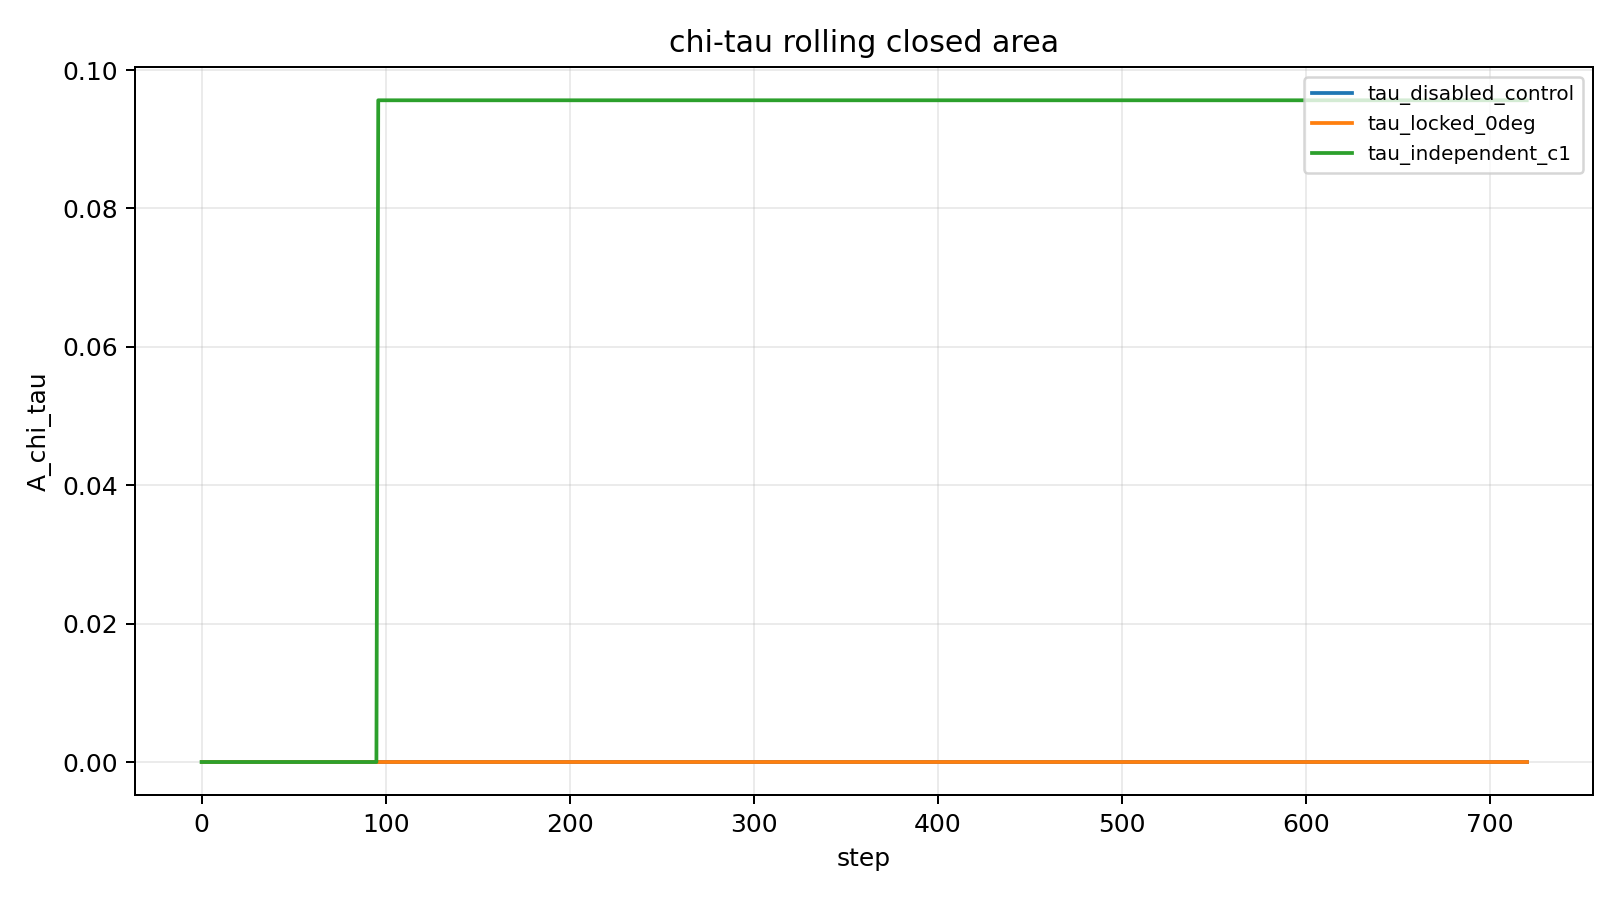
\includegraphics[keepaspectratio,alt={figure}]{ab_two_body_c1_internal_calibration_chi_tau_area_sweep_preliminary_result_v1/ab_two_body_c1_internal_calibration_area_sweep_v1.png}} \\
\end{longtable}
}

{\def\LTcaptype{none} % do not increment counter
\begin{longtable}[]{@{}
  >{\raggedright\arraybackslash}p{(\linewidth - 2\tabcolsep) * \real{0.5000}}
  >{\raggedright\arraybackslash}p{(\linewidth - 2\tabcolsep) * \real{0.5000}}@{}}
\toprule\noalign{}
\begin{minipage}[b]{\linewidth}\raggedright
\texttt{c=1} calibration error
\end{minipage} & \begin{minipage}[b]{\linewidth}\raggedright
Power candidates
\end{minipage} \\
\midrule\noalign{}
\endhead
\bottomrule\noalign{}
\endlastfoot
\pandocbounded{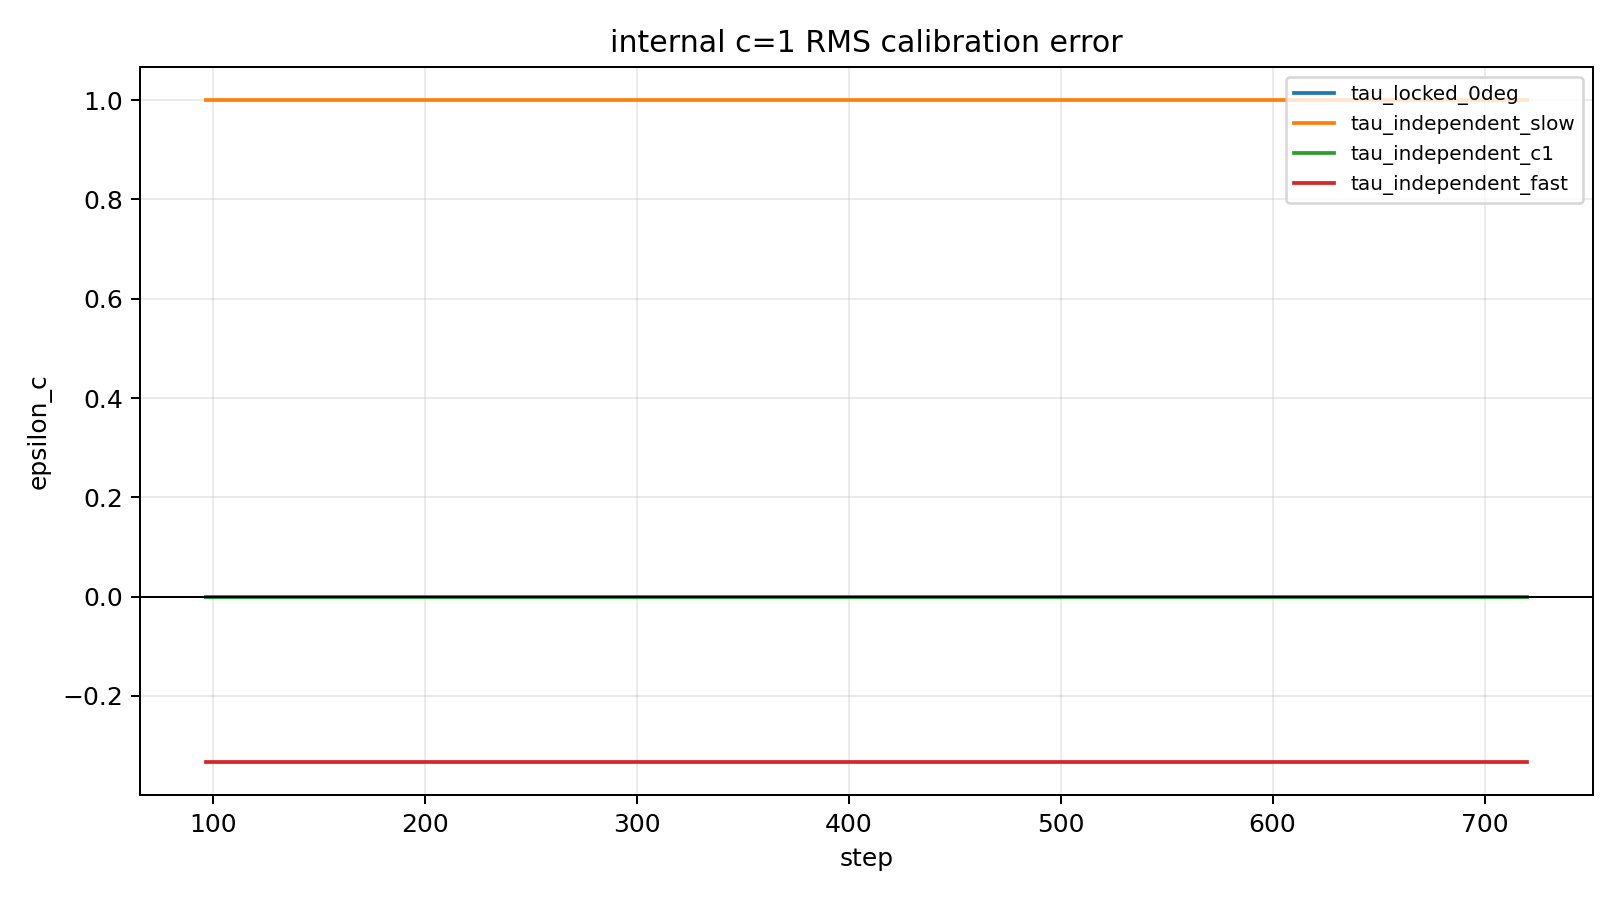
\includegraphics[keepaspectratio,alt={figure}]{ab_two_body_c1_internal_calibration_chi_tau_area_sweep_preliminary_result_v1/ab_two_body_c1_internal_calibration_error_v1.png}}
&
\pandocbounded{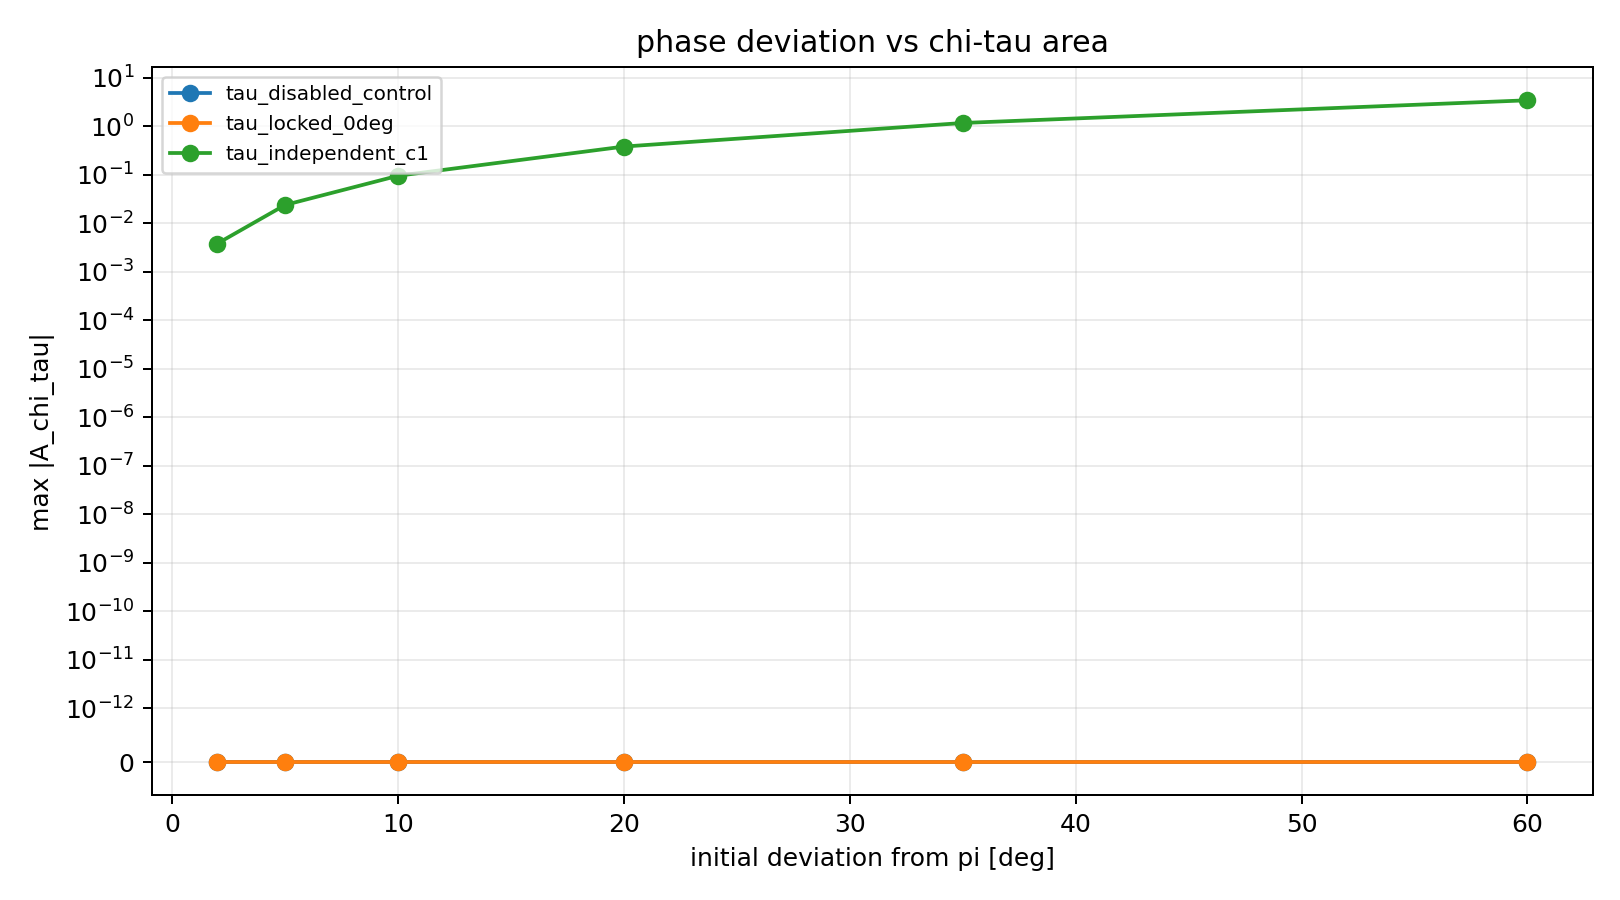
\includegraphics[keepaspectratio,alt={figure}]{ab_two_body_c1_internal_calibration_chi_tau_area_sweep_preliminary_result_v1/ab_two_body_c1_internal_calibration_power_candidate_v1.png}} \\
\end{longtable}
}

{\def\LTcaptype{none} % do not increment counter
\begin{longtable}[]{@{}
  >{\raggedright\arraybackslash}p{(\linewidth - 0\tabcolsep) * \real{1.0000}}@{}}
\toprule\noalign{}
\begin{minipage}[b]{\linewidth}\raggedright
Readout leakage
\end{minipage} \\
\midrule\noalign{}
\endhead
\bottomrule\noalign{}
\endlastfoot
\pandocbounded{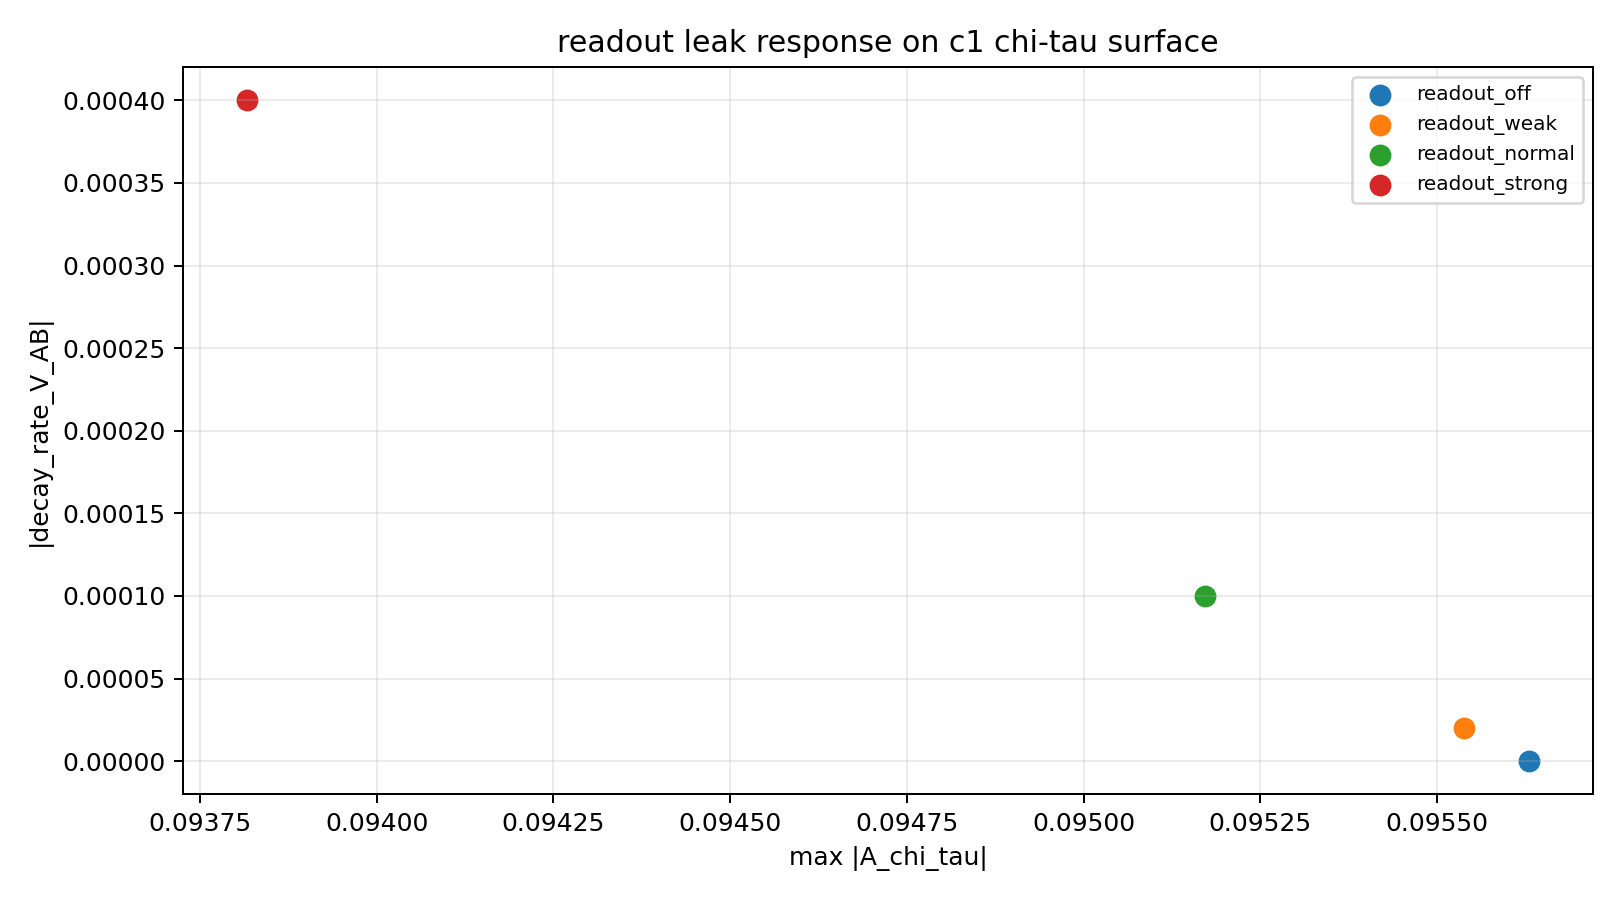
\includegraphics[keepaspectratio,alt={figure}]{ab_two_body_c1_internal_calibration_chi_tau_area_sweep_preliminary_result_v1/ab_two_body_c1_internal_calibration_readout_leak_v1.png}} \\
\end{longtable}
}

\begin{center}\rule{0.5\linewidth}{0.5pt}\end{center}

\subsection{5. c=1 Internal Calibration Parameter
Sweep}\label{c1-internal-calibration-parameter-sweep}

\subsubsection{5.1 Main Result}\label{main-result-3}

{\def\LTcaptype{none} % do not increment counter
\begin{longtable}[]{@{}lr@{}}
\toprule\noalign{}
Quantity & Value \\
\midrule\noalign{}
\endhead
\bottomrule\noalign{}
\endlastfoot
\texttt{sweep\_case\_count} & \texttt{756} \\
\texttt{readout\_off\_case\_count} & \texttt{252} \\
\texttt{rank2\_readout\_off\_count} & \texttt{246} \\
\texttt{c1\_surface\_like\_readout\_off\_count} & \texttt{13} \\
\texttt{c1\_locked\_like\_readout\_off\_count} & \texttt{8} \\
\texttt{min\_c\_error\_readout\_off} & \texttt{1.11e-15} \\
\texttt{max\_area\_readout\_off} & \texttt{0.19685536479742288} \\
\end{longtable}
}

This clarified that the following three conditions must be required
simultaneously:

\begin{Shaded}
\begin{Highlighting}[]
\NormalTok{c=1}
\NormalTok{rank\_chi\_tau = 2}
\NormalTok{A\_chi\_tau != 0}
\end{Highlighting}
\end{Shaded}

Being close to \texttt{c=1} alone does not mean that a \texttt{chi-tau}
surface has been formed.

{\def\LTcaptype{none} % do not increment counter
\begin{longtable}[]{@{}
  >{\raggedright\arraybackslash}p{(\linewidth - 2\tabcolsep) * \real{0.5000}}
  >{\raggedright\arraybackslash}p{(\linewidth - 2\tabcolsep) * \real{0.5000}}@{}}
\toprule\noalign{}
\begin{minipage}[b]{\linewidth}\raggedright
c-error heatmap
\end{minipage} & \begin{minipage}[b]{\linewidth}\raggedright
Area heatmap
\end{minipage} \\
\midrule\noalign{}
\endhead
\bottomrule\noalign{}
\endlastfoot
\pandocbounded{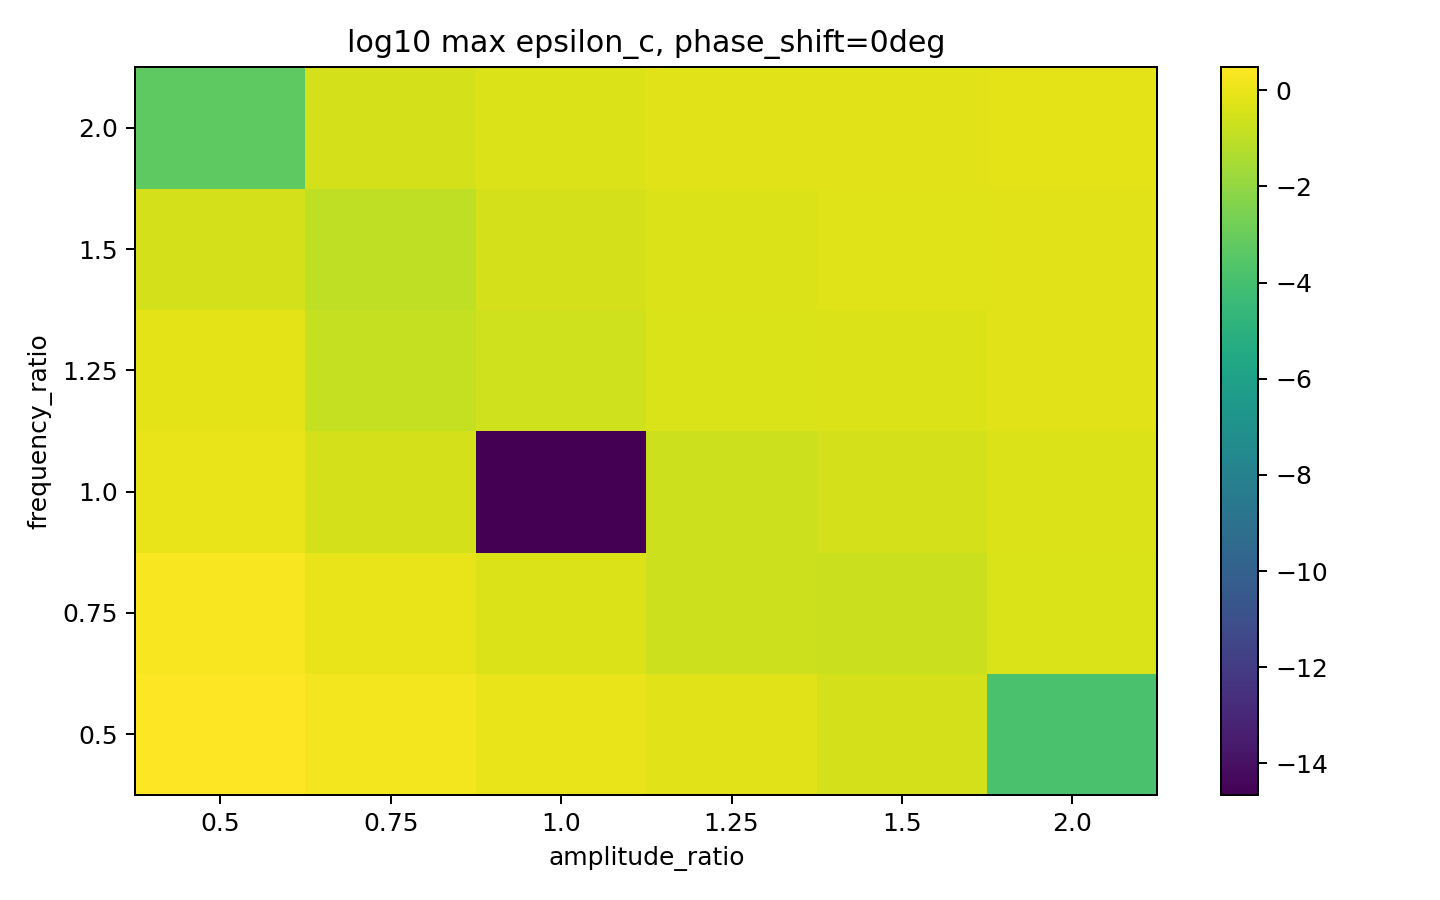
\includegraphics[keepaspectratio,alt={figure}]{ab_two_body_c1_internal_calibration_parameter_sweep_preliminary_result_v1/ab_two_body_c1_parameter_sweep_c_error_heatmap_v1.png}}
&
\pandocbounded{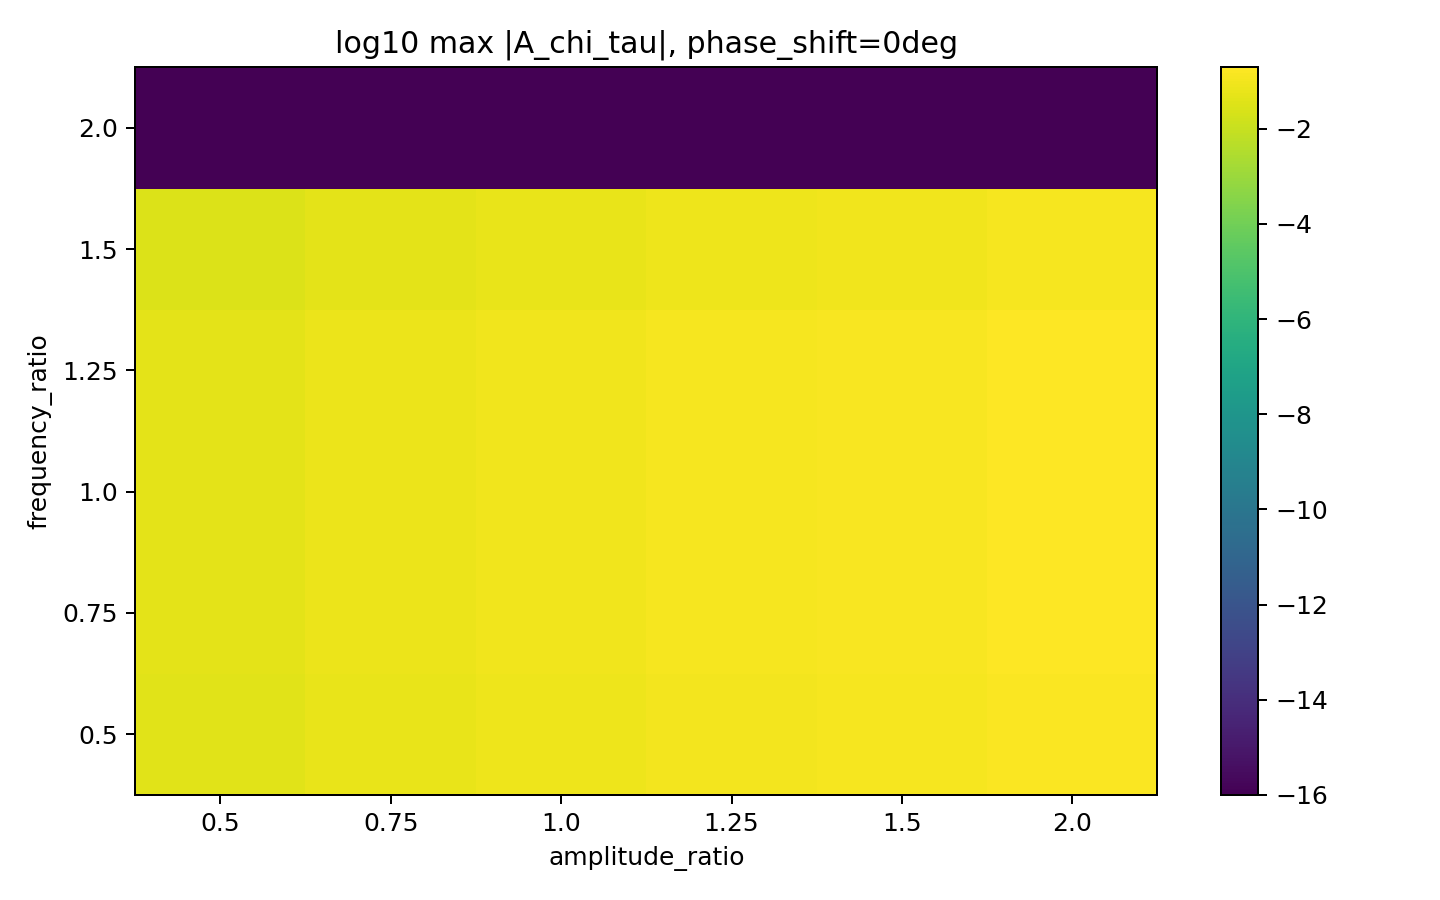
\includegraphics[keepaspectratio,alt={figure}]{ab_two_body_c1_internal_calibration_parameter_sweep_preliminary_result_v1/ab_two_body_c1_parameter_sweep_area_heatmap_v1.png}} \\
\end{longtable}
}

{\def\LTcaptype{none} % do not increment counter
\begin{longtable}[]{@{}
  >{\raggedright\arraybackslash}p{(\linewidth - 2\tabcolsep) * \real{0.5000}}
  >{\raggedright\arraybackslash}p{(\linewidth - 2\tabcolsep) * \real{0.5000}}@{}}
\toprule\noalign{}
\begin{minipage}[b]{\linewidth}\raggedright
Phase-difference response
\end{minipage} & \begin{minipage}[b]{\linewidth}\raggedright
Readout leakage
\end{minipage} \\
\midrule\noalign{}
\endhead
\bottomrule\noalign{}
\endlastfoot
\pandocbounded{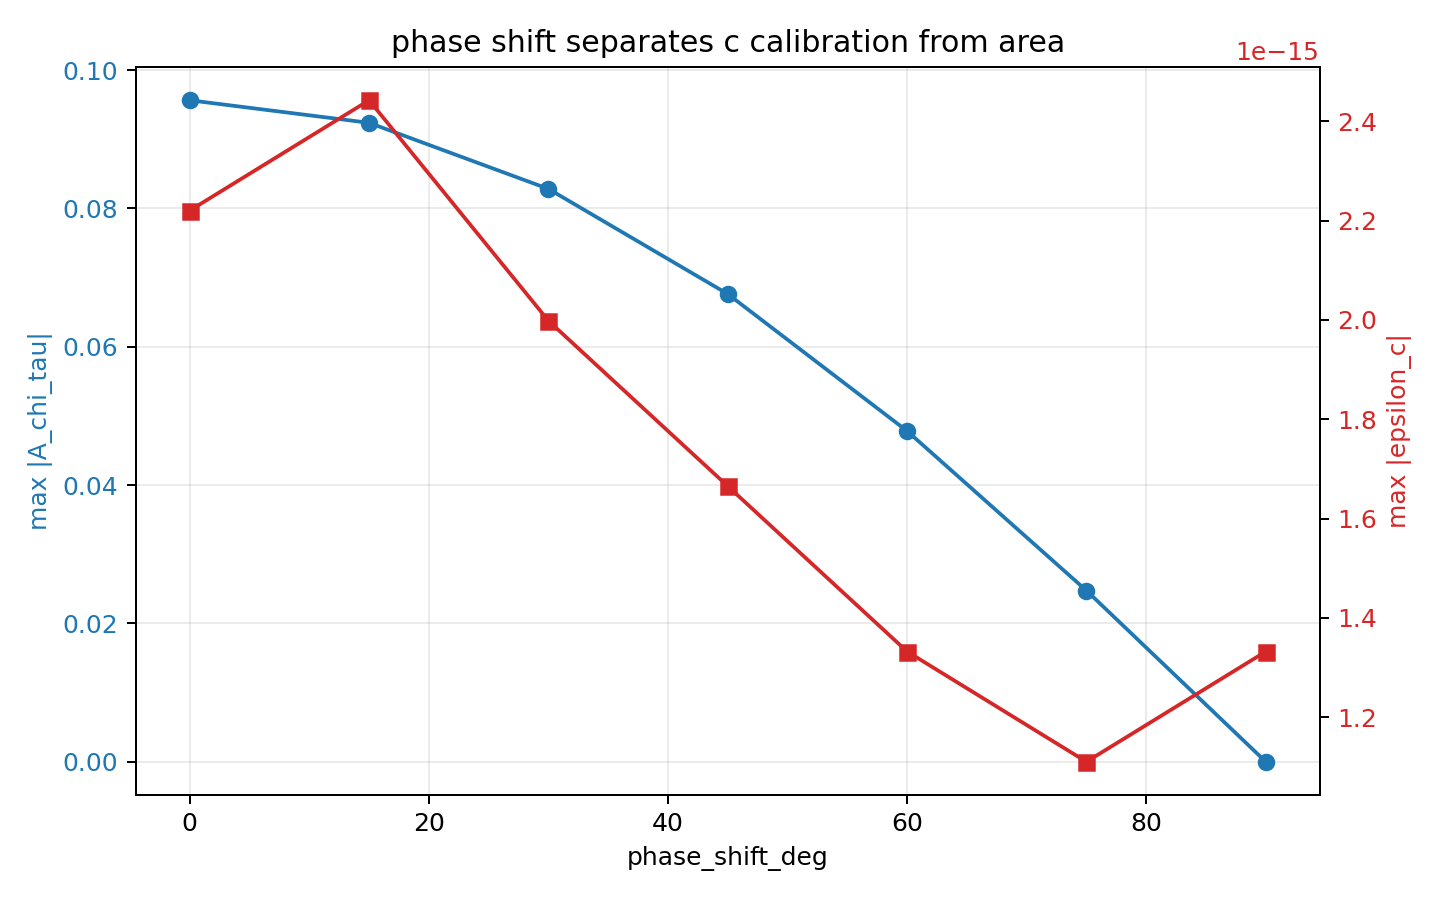
\includegraphics[keepaspectratio,alt={figure}]{ab_two_body_c1_internal_calibration_parameter_sweep_preliminary_result_v1/ab_two_body_c1_parameter_sweep_phase_response_v1.png}}
&
\pandocbounded{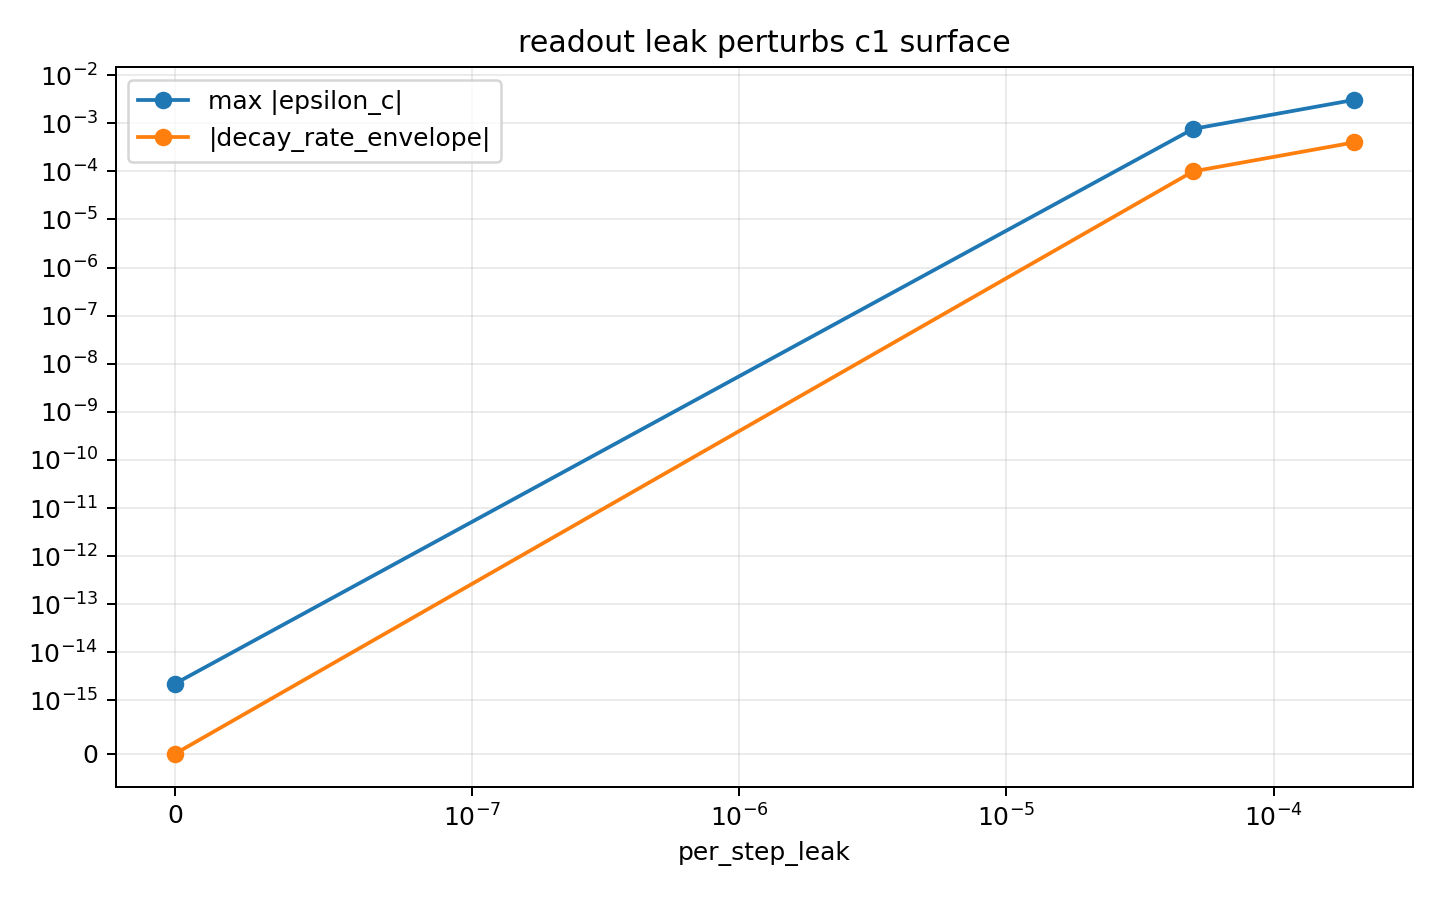
\includegraphics[keepaspectratio,alt={figure}]{ab_two_body_c1_internal_calibration_parameter_sweep_preliminary_result_v1/ab_two_body_c1_parameter_sweep_readout_leak_v1.png}} \\
\end{longtable}
}

\begin{center}\rule{0.5\linewidth}{0.5pt}\end{center}

\subsection{6. Inverse-Area Compensation
Diagnosis}\label{inverse-area-compensation-diagnosis}

\subsubsection{6.1 Purpose}\label{purpose}

After the \texttt{chi-tau} area was formed, the experiment tested
whether

\begin{Shaded}
\begin{Highlighting}[]
\NormalTok{1 / A\_chi\_tau}
\end{Highlighting}
\end{Shaded}

would naturally remain on the closure-compensation side.

The important point is not to construct \texttt{1/A\_chi\_tau} as
post-processing.

That is a constructed control and must be distinguished from native
readout.

\subsubsection{6.2 Main Result}\label{main-result-4}

{\def\LTcaptype{none} % do not increment counter
\begin{longtable}[]{@{}lr@{}}
\toprule\noalign{}
Quantity & Value \\
\midrule\noalign{}
\endhead
\bottomrule\noalign{}
\endlastfoot
\texttt{diagnostic\_case\_count} & \texttt{288} \\
\texttt{area\_valid\_case\_count} & \texttt{144} \\
\texttt{fit\_count} & \texttt{576} \\
\texttt{native\_fit\_count} & \texttt{132} \\
\texttt{derived\_fit\_count} & \texttt{84} \\
\texttt{native\_positive2\_count} & \texttt{0} \\
\texttt{constructed\_reciprocal\_positive2\_count} & \texttt{2} \\
\end{longtable}
}

The result is clear.

\begin{Shaded}
\begin{Highlighting}[]
\NormalTok{If 1 / A\_chi\_tau is constructed, alpha≈2 appears.}
\NormalTok{However, alpha≈2 does not appear in native readout.}
\end{Highlighting}
\end{Shaded}

{\def\LTcaptype{none} % do not increment counter
\begin{longtable}[]{@{}
  >{\raggedright\arraybackslash}p{(\linewidth - 2\tabcolsep) * \real{0.5000}}
  >{\raggedright\arraybackslash}p{(\linewidth - 2\tabcolsep) * \real{0.5000}}@{}}
\toprule\noalign{}
\begin{minipage}[b]{\linewidth}\raggedright
Constructed inverse-area control
\end{minipage} & \begin{minipage}[b]{\linewidth}\raggedright
Native candidates
\end{minipage} \\
\midrule\noalign{}
\endhead
\bottomrule\noalign{}
\endlastfoot
\pandocbounded{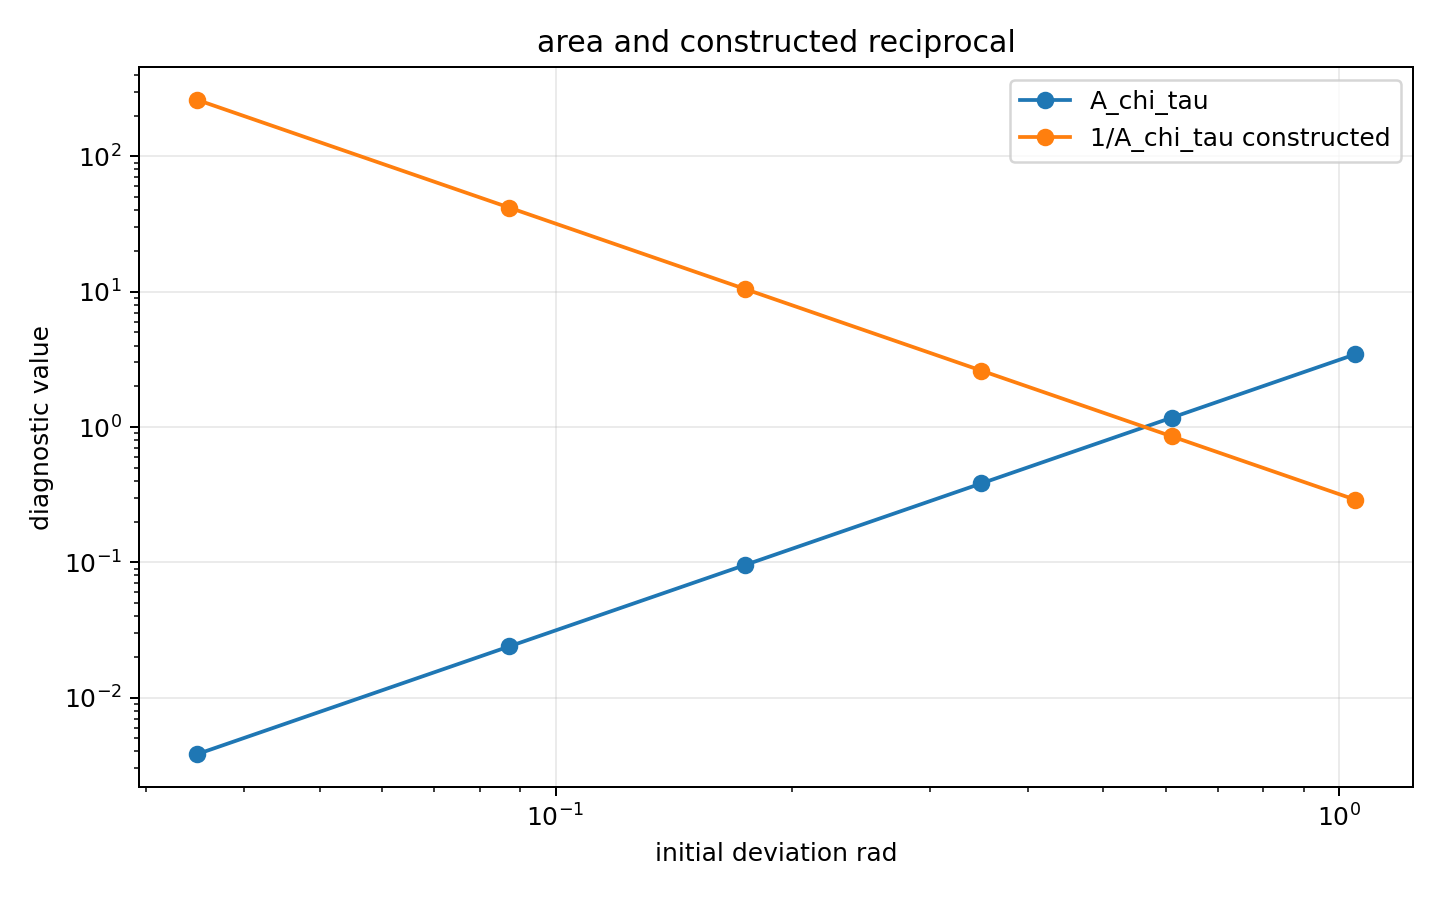
\includegraphics[keepaspectratio,alt={figure}]{ab_two_body_chi_tau_inverse_area_compensation_diagnostic_preliminary_result_v1/ab_two_body_chi_tau_inverse_area_constructed_control_v1.png}}
&
\pandocbounded{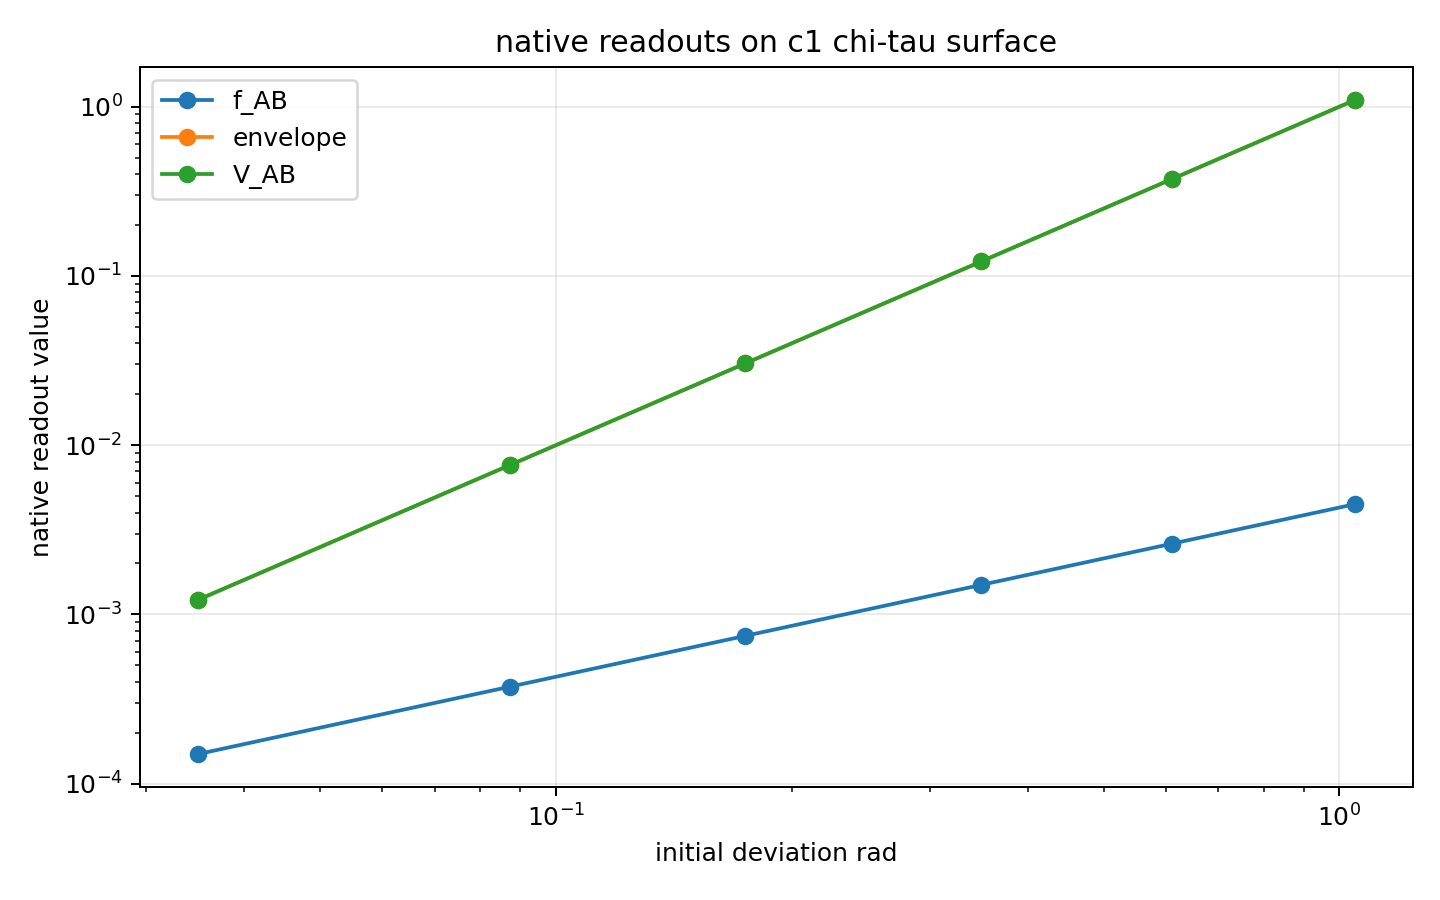
\includegraphics[keepaspectratio,alt={figure}]{ab_two_body_chi_tau_inverse_area_compensation_diagnostic_preliminary_result_v1/ab_two_body_chi_tau_inverse_area_native_candidates_v1.png}} \\
\end{longtable}
}

{\def\LTcaptype{none} % do not increment counter
\begin{longtable}[]{@{}
  >{\raggedright\arraybackslash}p{(\linewidth - 0\tabcolsep) * \real{1.0000}}@{}}
\toprule\noalign{}
\begin{minipage}[b]{\linewidth}\raggedright
Alpha comparison
\end{minipage} \\
\midrule\noalign{}
\endhead
\bottomrule\noalign{}
\endlastfoot
\pandocbounded{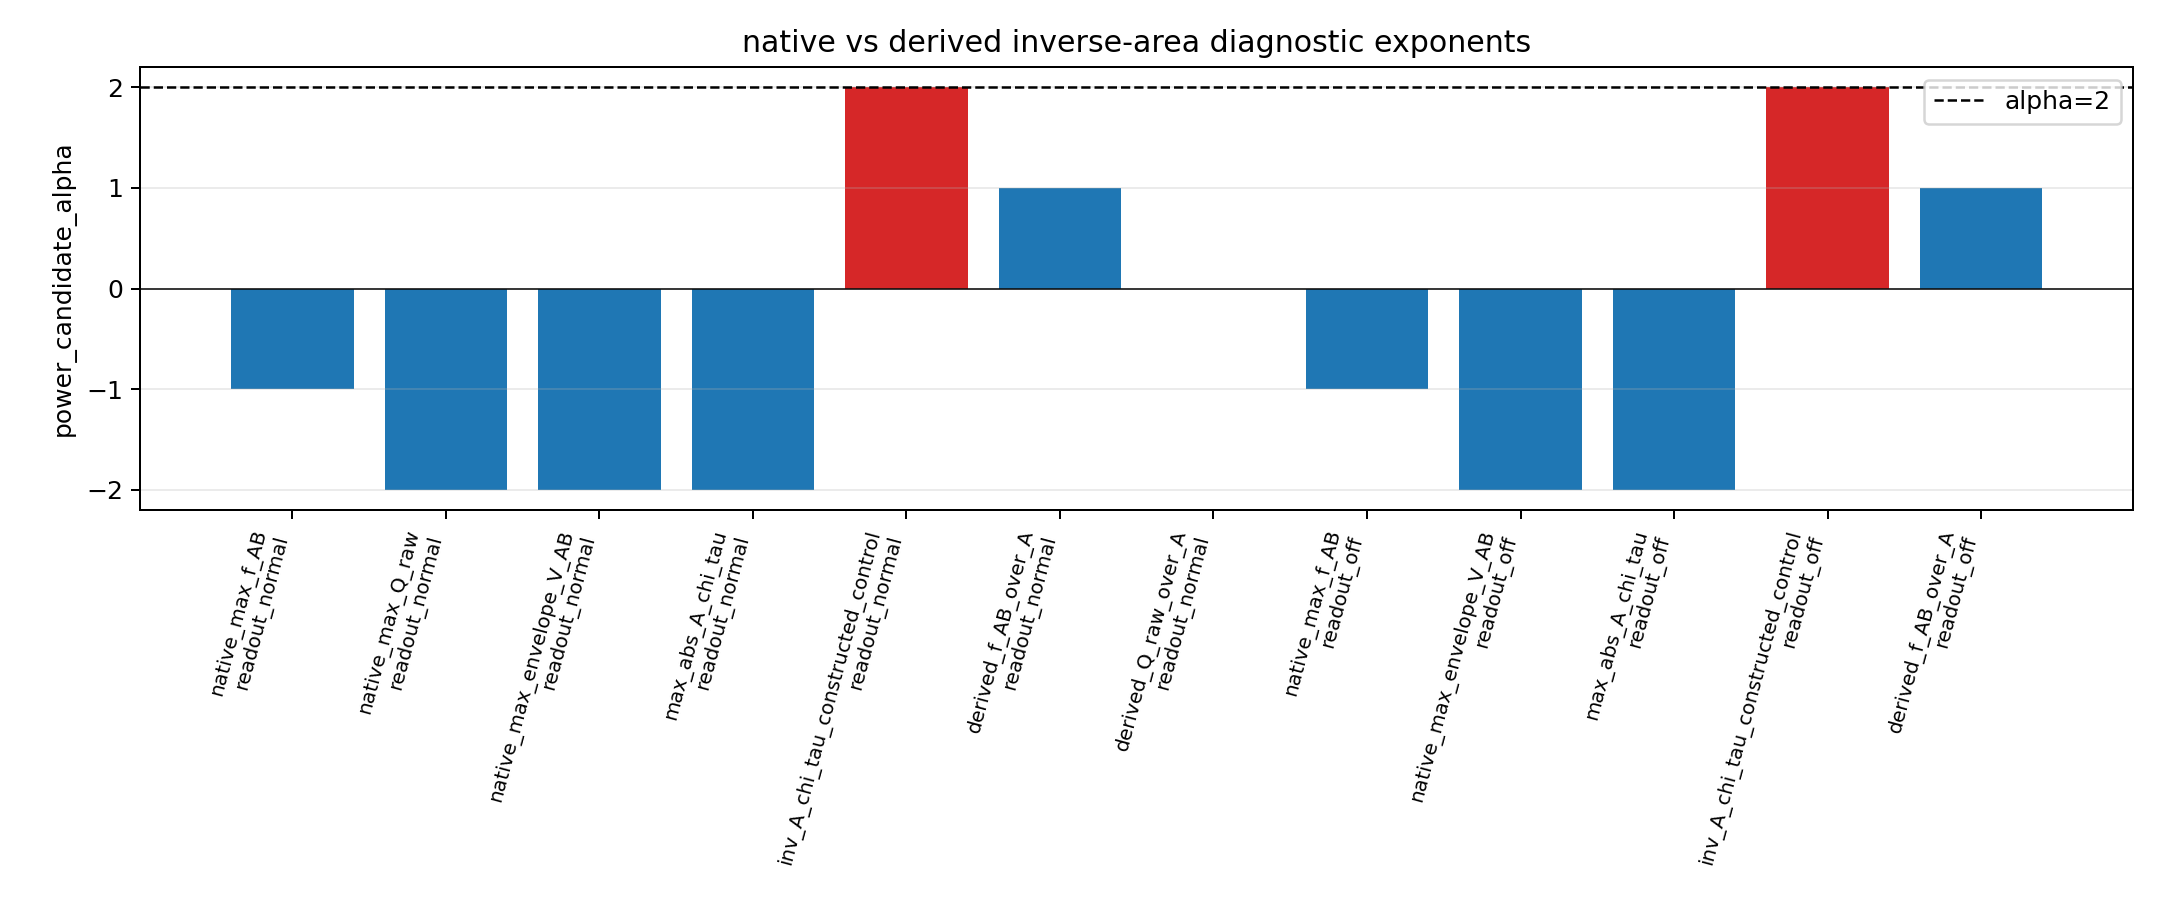
\includegraphics[keepaspectratio,alt={figure}]{ab_two_body_chi_tau_inverse_area_compensation_diagnostic_preliminary_result_v1/ab_two_body_chi_tau_inverse_area_alpha_comparison_v1.png}} \\
\end{longtable}
}

\begin{center}\rule{0.5\linewidth}{0.5pt}\end{center}

\subsection{7. Native Inverse-Area Extended
Sweep}\label{native-inverse-area-extended-sweep}

\subsubsection{7.1 Main Result}\label{main-result-5}

{\def\LTcaptype{none} % do not increment counter
\begin{longtable}[]{@{}lr@{}}
\toprule\noalign{}
Quantity & Value \\
\midrule\noalign{}
\endhead
\bottomrule\noalign{}
\endlastfoot
\texttt{sweep\_case\_count} & \texttt{1323} \\
\texttt{area\_valid\_case\_count} & \texttt{1260} \\
\texttt{c1\_surface\_like\_case\_count} & \texttt{126} \\
\texttt{fit\_count} & \texttt{4158} \\
\texttt{native\_fit\_count} & \texttt{1056} \\
\texttt{native\_positive2\_count} & \texttt{0} \\
\texttt{c1\_native\_positive2\_count} & \texttt{0} \\
\texttt{constructed\_reciprocal\_positive2\_count} & \texttt{198} \\
\end{longtable}
}

Across a broad parameter range,

\begin{Shaded}
\begin{Highlighting}[]
\NormalTok{native inverse{-}area scaling was not detected.}
\end{Highlighting}
\end{Shaded}

On the other hand, the constructed control does produce
\texttt{alpha≈2}.

Thus the boundary found here is:

\begin{Shaded}
\begin{Highlighting}[]
\NormalTok{The inverse{-}square form can be constructed.}
\NormalTok{However, it has not yet been read natively.}
\end{Highlighting}
\end{Shaded}

{\def\LTcaptype{none} % do not increment counter
\begin{longtable}[]{@{}
  >{\raggedright\arraybackslash}p{(\linewidth - 2\tabcolsep) * \real{0.5000}}
  >{\raggedright\arraybackslash}p{(\linewidth - 2\tabcolsep) * \real{0.5000}}@{}}
\toprule\noalign{}
\begin{minipage}[b]{\linewidth}\raggedright
Reference curves
\end{minipage} & \begin{minipage}[b]{\linewidth}\raggedright
Alpha scan
\end{minipage} \\
\midrule\noalign{}
\endhead
\bottomrule\noalign{}
\endlastfoot
\pandocbounded{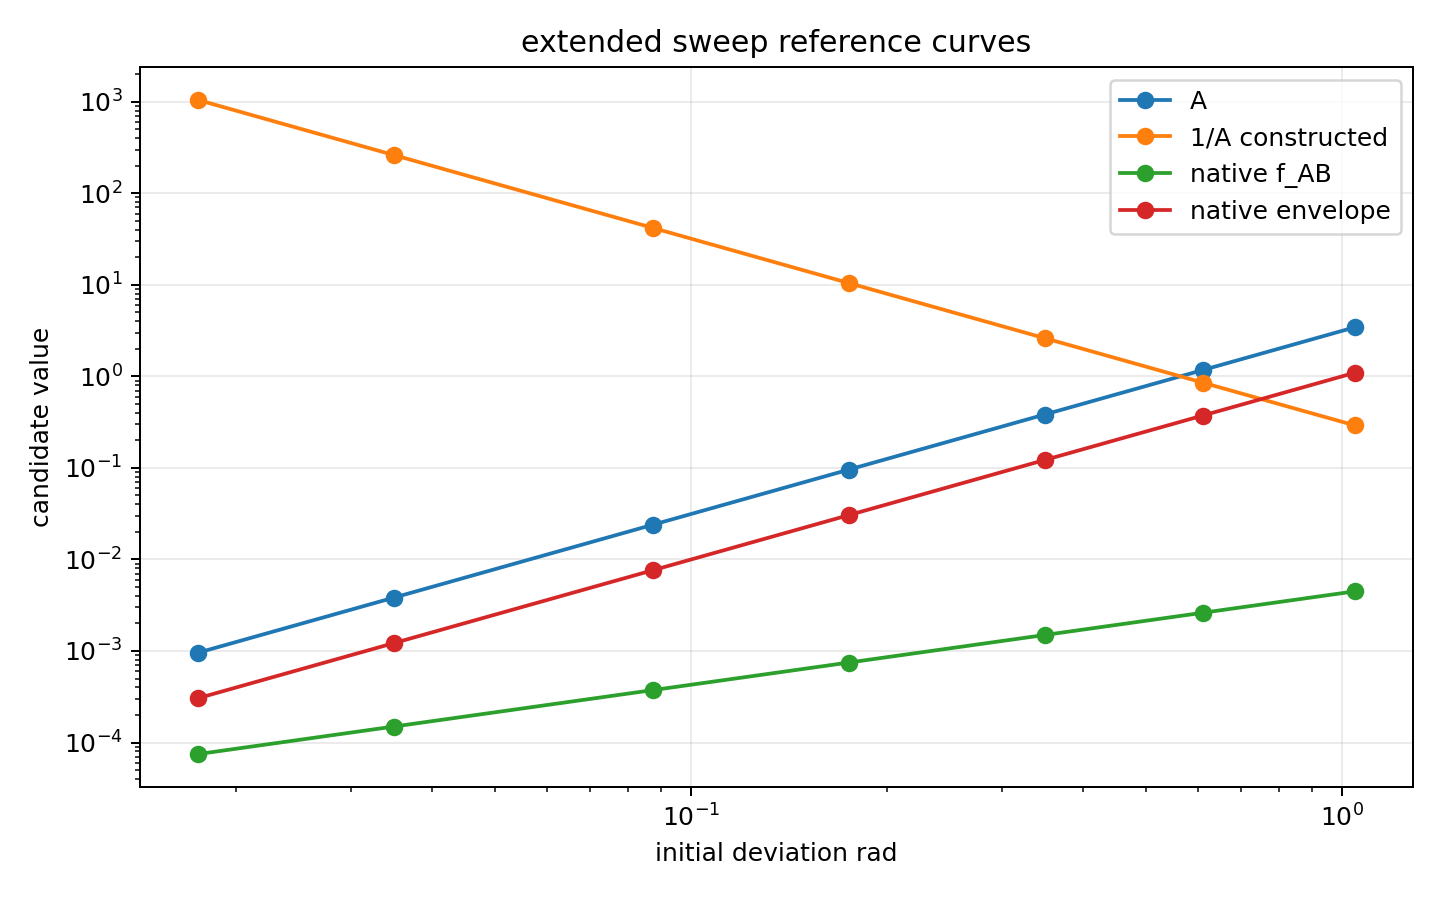
\includegraphics[keepaspectratio,alt={figure}]{ab_two_body_chi_tau_native_inverse_area_extended_sweep_preliminary_result_v1/ab_two_body_native_inverse_area_extended_reference_curves_v1.png}}
&
\pandocbounded{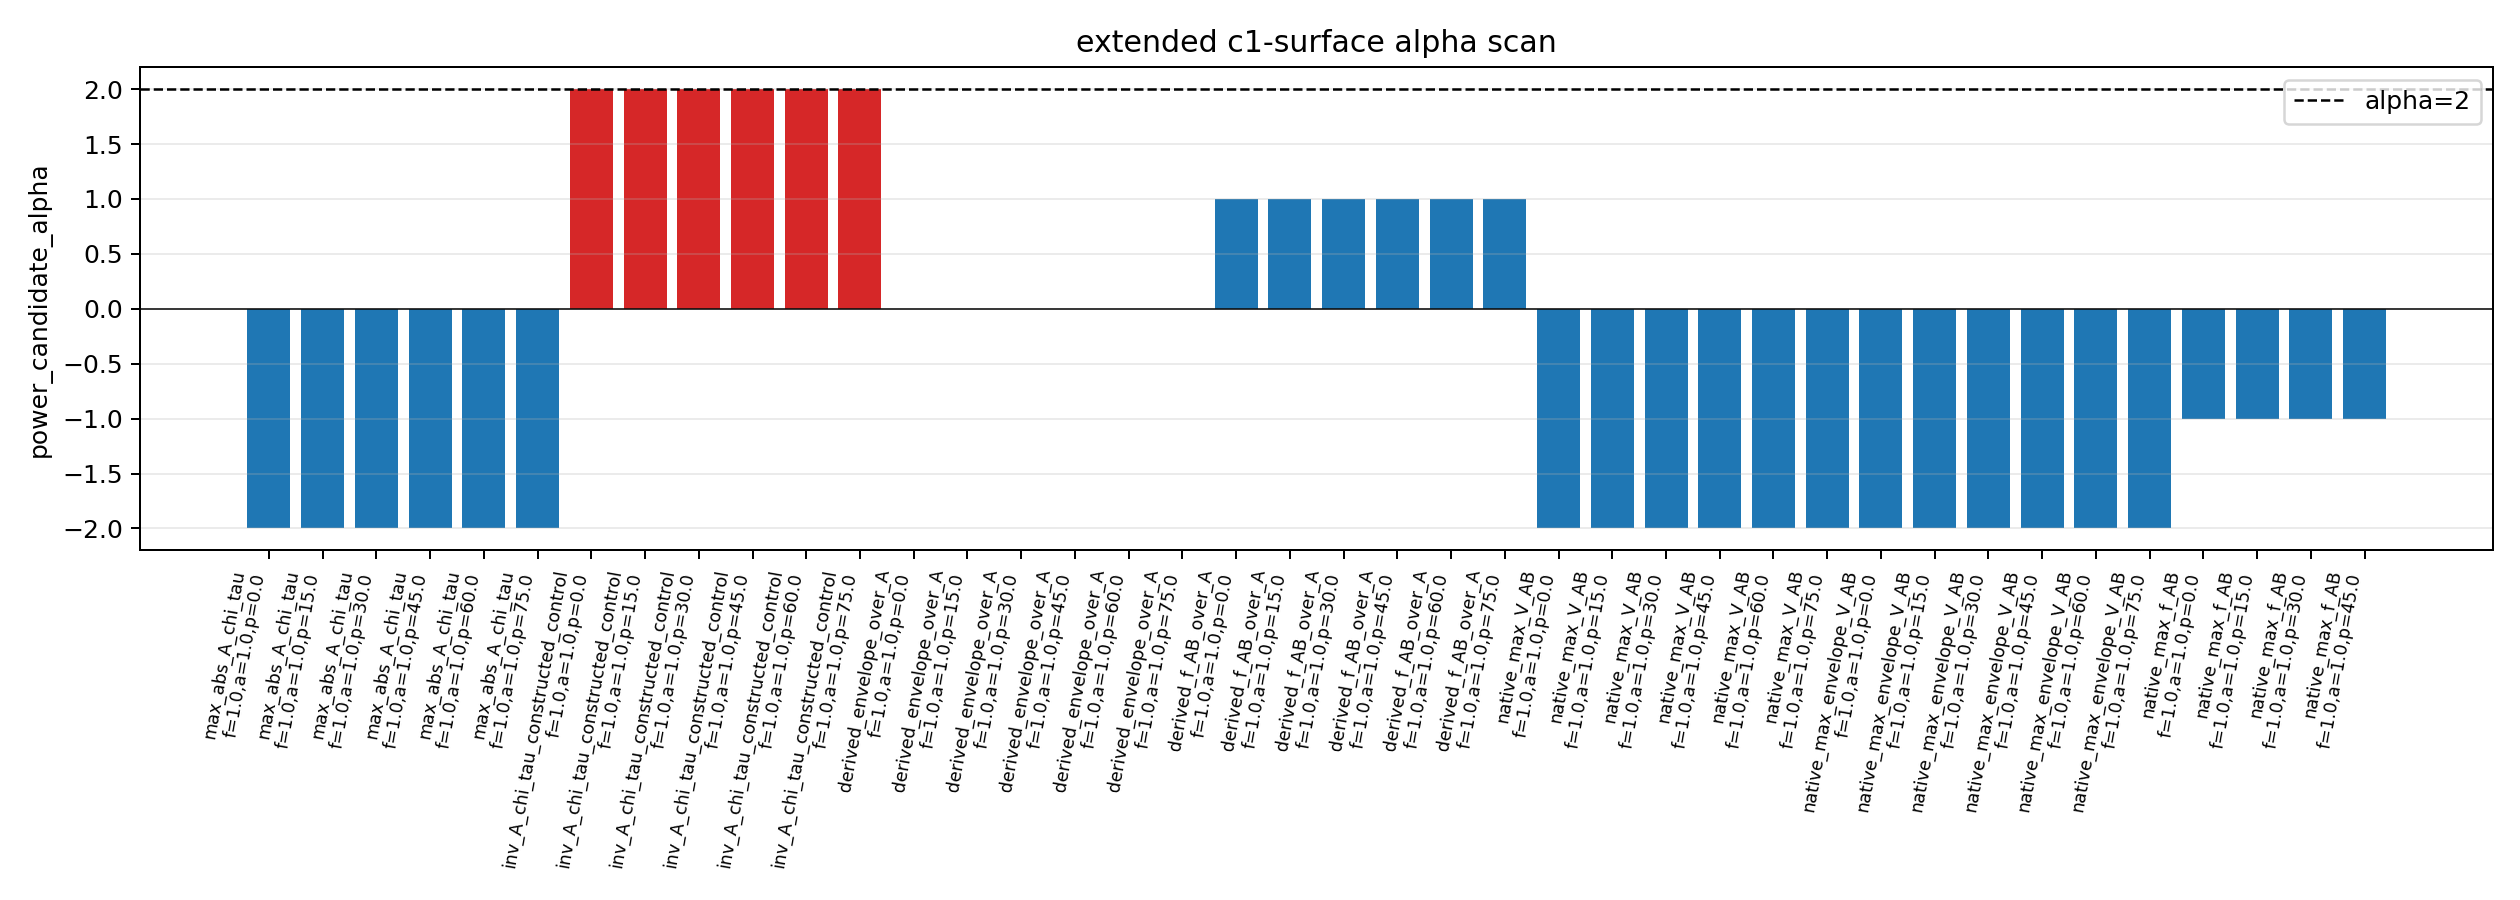
\includegraphics[keepaspectratio,alt={figure}]{ab_two_body_chi_tau_native_inverse_area_extended_sweep_preliminary_result_v1/ab_two_body_native_inverse_area_extended_alpha_scan_v1.png}} \\
\end{longtable}
}

\begin{center}\rule{0.5\linewidth}{0.5pt}\end{center}

\subsection{8. V3 Addition: Harmonic Readout with a Fermion-Like Recoil
Map}\label{v3-addition-harmonic-readout-with-a-fermion-like-recoil-map}

\subsubsection{8.1 Purpose}\label{purpose-1}

In the V1 one-angle harmonic readout, the relative phase development of
the AB pair was read continuously, and Protocol F/B degeneracy was
confirmed under label-free readout.

V3 keeps this context unchanged and adds a fermion-like recoil map at
the central interaction region.

The implementation change is limited to one readout operation:

\begin{Shaded}
\begin{Highlighting}[]
\NormalTok{chi\_read = q\_out\_factor * chi\_pass}
\NormalTok{q\_out\_factor = T {-} R}
\end{Highlighting}
\end{Shaded}

Under the complete-recoil condition, \texttt{R=1} and \texttt{T≈0}, so
\texttt{q\_out\_factor=-1}.

The question tested here is whether the acceleration-like harmonic
readout from the AB two-body relation \texttt{f\_AB} can still be
evaluated in the same form when the central interaction is read as a
recoil-type event.

This section does not test:

\begin{Shaded}
\begin{Highlighting}[]
\NormalTok{AB asymmetrization}
\NormalTok{low{-}localization limit}
\NormalTok{instantaneous contraction}
\NormalTok{harmonic transfer}
\NormalTok{localization transfer}
\end{Highlighting}
\end{Shaded}

Those questions belong to a separate wave-packet focusing experiment
line.

The present V3 evaluates the fermion-like recoil protocol within the
current AB two-body acceleration-readout assumptions, in addition to the
transmission-type central readout.

\subsubsection{8.2 Recoil Map}\label{recoil-map}

Let the right-moving and left-moving incident channels be

\begin{Shaded}
\begin{Highlighting}[]
\NormalTok{\textbackslash{}Psi\^{}\{\textbackslash{}mathrm\{in\}\}}
\NormalTok{=}
\NormalTok{\textbackslash{}begin\{pmatrix\}}
\NormalTok{\textbackslash{}psi\_+\^{}\{\textbackslash{}mathrm\{in\}\}\textbackslash{}\textbackslash{}}
\NormalTok{\textbackslash{}psi\_{-}\^{}\{\textbackslash{}mathrm\{in\}\}}
\NormalTok{\textbackslash{}end\{pmatrix\}.}
\end{Highlighting}
\end{Shaded}

Let \texttt{Delta\_F} be the fermion-like exchange phase. Define the
transmission and reflection amplitudes by

\begin{Shaded}
\begin{Highlighting}[]
\NormalTok{t\_\textbackslash{}Delta}
\NormalTok{=}
\NormalTok{e\^{}\{i\textbackslash{}Delta\_F/2\}}
\NormalTok{\textbackslash{}cos\textbackslash{}frac\{\textbackslash{}Delta\_F\}\{2\}}
\end{Highlighting}
\end{Shaded}

\begin{Shaded}
\begin{Highlighting}[]
\NormalTok{r\_\textbackslash{}Delta}
\NormalTok{=}
\NormalTok{{-}i e\^{}\{i\textbackslash{}Delta\_F/2\}}
\NormalTok{\textbackslash{}sin\textbackslash{}frac\{\textbackslash{}Delta\_F\}\{2\}.}
\end{Highlighting}
\end{Shaded}

The two-channel scattering matrix is

\begin{Shaded}
\begin{Highlighting}[]
\NormalTok{S\_\textbackslash{}Delta}
\NormalTok{=}
\NormalTok{\textbackslash{}begin\{pmatrix\}}
\NormalTok{t\_\textbackslash{}Delta \& r\_\textbackslash{}Delta\textbackslash{}\textbackslash{}}
\NormalTok{r\_\textbackslash{}Delta \& t\_\textbackslash{}Delta}
\NormalTok{\textbackslash{}end\{pmatrix\},}
\end{Highlighting}
\end{Shaded}

and the outgoing channels are read as

\begin{Shaded}
\begin{Highlighting}[]
\NormalTok{\textbackslash{}Psi\^{}\{\textbackslash{}mathrm\{out\}\}}
\NormalTok{=}
\NormalTok{S\_\textbackslash{}Delta}
\NormalTok{\textbackslash{}Psi\^{}\{\textbackslash{}mathrm\{in\}\}.}
\end{Highlighting}
\end{Shaded}

For the complete-recoil condition,

\begin{Shaded}
\begin{Highlighting}[]
\NormalTok{\textbackslash{}Delta\_F=\textbackslash{}pi,}
\end{Highlighting}
\end{Shaded}

we obtain

\begin{Shaded}
\begin{Highlighting}[]
\NormalTok{|r\_\textbackslash{}Delta|\^{}2=1,}
\NormalTok{\textbackslash{}qquad}
\NormalTok{|t\_\textbackslash{}Delta|\^{}2=0.}
\end{Highlighting}
\end{Shaded}

In this limit the readout factor becomes

\begin{Shaded}
\begin{Highlighting}[]
\NormalTok{q\_out\_factor = T {-} R = {-}1.}
\end{Highlighting}
\end{Shaded}

\subsubsection{8.3 Result}\label{result}

The V3 protocol preserved the same harmonic-readout frame.

\begin{Shaded}
\begin{Highlighting}[]
\NormalTok{q\_out\_factor = {-}1}
\end{Highlighting}
\end{Shaded}

The factor was applied to \texttt{chi\_read}. The AB harmonic readout
remained evaluable in the same form, and the \texttt{chi-tau} surface
used in the area sweep was maintained.

This result does not add a claim of immediate contraction, harmonic
transfer, or localization transfer. It only confirms that the
acceleration-like AB readout survives when the central interaction is
represented as a fermion-like recoil map.

\subsection{9. Overall Judgment}\label{overall-judgment}

\subsubsection{9.1 Established}\label{established}

{\def\LTcaptype{none} % do not increment counter
\begin{longtable}[]{@{}
  >{\raggedright\arraybackslash}p{(\linewidth - 2\tabcolsep) * \real{0.5000}}
  >{\raggedright\arraybackslash}p{(\linewidth - 2\tabcolsep) * \real{0.5000}}@{}}
\toprule\noalign{}
\begin{minipage}[b]{\linewidth}\raggedright
Item
\end{minipage} & \begin{minipage}[b]{\linewidth}\raggedright
Judgment
\end{minipage} \\
\midrule\noalign{}
\endhead
\bottomrule\noalign{}
\endlastfoot
Read \texttt{f\_AB} as a single AB relation & Established \\
Read harmonic oscillation without placing \texttt{f\_A} or \texttt{f\_B}
& Established \\
Confirm label-free degeneracy of Protocol F/B & Established \\
Confirm disappearance of decay when the readout wave is stopped &
Established \\
Read \texttt{chi-tau} area through independent \texttt{tau\_read} &
Established \\
Confirm \texttt{c=1} as a candidate necessary condition & Established \\
Post-processed \texttt{1/A\_chi\_tau} shows \texttt{alpha≈2} &
Established \\
\end{longtable}
}

\subsubsection{9.2 Not Established}\label{not-established}

{\def\LTcaptype{none} % do not increment counter
\begin{longtable}[]{@{}
  >{\raggedright\arraybackslash}p{(\linewidth - 2\tabcolsep) * \real{0.5000}}
  >{\raggedright\arraybackslash}p{(\linewidth - 2\tabcolsep) * \real{0.5000}}@{}}
\toprule\noalign{}
\begin{minipage}[b]{\linewidth}\raggedright
Item
\end{minipage} & \begin{minipage}[b]{\linewidth}\raggedright
Judgment
\end{minipage} \\
\midrule\noalign{}
\endhead
\bottomrule\noalign{}
\endlastfoot
Independent metrical determination of distance exponent in AB two-body
system alone & Not established \\
Formation of temporal phase surface from \texttt{c=1} alone & Not
established \\
Native inverse-law readout & Not detected \\
Native inverse-square readout & Not detected \\
Automatic conversion from \texttt{chi-tau} area to \texttt{1/A}
compensation & Not detected \\
Correspondence to standard gravity & Not established \\
\end{longtable}
}

\begin{center}\rule{0.5\linewidth}{0.5pt}\end{center}

\subsection{10. Interpretation}\label{interpretation}

The main achievements of the AB two-body system are the following two
points:

\begin{Shaded}
\begin{Highlighting}[]
\NormalTok{1. Using only the AB relation f\_AB, an acceleration{-}like harmonic readout can be constructed.}
\NormalTok{2. The AB two{-}body system alone lacks an independent gauge for reading the distance exponent.}
\end{Highlighting}
\end{Shaded}

The first point is a positive result.

In the preceding ABC multigauge interference readout experiment,
mass-like, momentum-like, and energy-like readouts were reconstructed
from interference correlations.

The present experiment shows, as a next step, that an acceleration-like
readout can be constructed from the harmonic AB two-body relation.

This is not the result of inserting a standard force from outside.

It is a harmonic displacement appearing as a closure readout of the
two-body relation \texttt{f\_AB}.

The second point is a boundary condition.

Inside the AB pair, A and B can be read only through one another.

Therefore, relative-distance change can be read, but there is no
independent gauge that fixes whether the change rate should be measured
as

\begin{Shaded}
\begin{Highlighting}[]
\NormalTok{proportional}
\NormalTok{inverse proportional}
\NormalTok{inverse square}
\end{Highlighting}
\end{Shaded}

This is not a failure of namelessness. Rather, it is a consequence of
namelessness.

What cannot be read must not be declared read by post-processing.

In the \texttt{chi-tau} area sweep, an independent temporal phase
allowed an area readout to stand.

However, this did not automatically provide a distance-exponent readout.

In addition, if \texttt{1/A\_chi\_tau} is constructed in
post-processing, an inverse-square form naturally appears. But this is
not native readout.

The judgment of this summary is therefore:

\begin{Shaded}
\begin{Highlighting}[]
\NormalTok{Acceleration{-}like readout was confirmed.}
\NormalTok{Distance{-}exponent readout cannot be determined in the AB two{-}body system alone.}
\end{Highlighting}
\end{Shaded}

\begin{center}\rule{0.5\linewidth}{0.5pt}\end{center}

\subsection{10. Connection to the Next
Experiment}\label{connection-to-the-next-experiment}

The next stage following this summary is the ABC three-body system.

However, the third wave \texttt{C} is not an external absolute observer.

\texttt{C} is itself part of the closed phase system and generates

\begin{Shaded}
\begin{Highlighting}[]
\NormalTok{f\_AC}
\NormalTok{f\_BC}
\NormalTok{f\_ABC}
\end{Highlighting}
\end{Shaded}

Therefore, the ABC experiment must test:

\begin{Shaded}
\begin{Highlighting}[]
\NormalTok{whether C can be used as an independent metrical gauge,}
\NormalTok{whether C contaminates the main AB readout,}
\NormalTok{whether f\_ABC can be used as representative time,}
\NormalTok{and whether f\_AB, f\_AC, and f\_BC can be separated as circumferential{-}direction candidates.}
\end{Highlighting}
\end{Shaded}

\begin{center}\rule{0.5\linewidth}{0.5pt}\end{center}

\section{References}\label{references}

\subsection{Self-References}\label{self-references}

\begin{enumerate}
\def\labelenumi{\arabic{enumi}.}
\tightlist
\item
  Noriaki Kihara, ``Basic Axiom System of the Nameless Equal-Amplitude
  Composite Wave Model v4'', Version DOI:
  \texttt{10.5281/zenodo.21316620}, Concept DOI:
  \texttt{10.5281/zenodo.21315735}, 2026.
\item
  Noriaki Kihara, ``Construction Experiment of Multigauge Interference
  Readout Conserved Quantities in an ABC Closed Phase System'', Version
  DOI: \texttt{10.5281/zenodo.21332875}, Concept DOI:
  \texttt{10.5281/zenodo.21308049}, 2026.
\item
  Noriaki Kihara,
  \href{AB二体閉鎖位相系におけるラベルなし二弧相対位相と調和読出しに関する定義補足.md}{Definitional
  Supplement on Label-Free Two-Arc Relative Phase and Harmonic Readout
  in an AB Two-Body Closed Phase System}, 2026.
\item
  Noriaki Kihara,
  \href{AB二体閉鎖位相系における一角度円周位相調和読出し実験仕様書\%20v1.md}{Experiment
  Specification for One-Angle Circumferential Phase Harmonic Readout in
  an AB Two-Body Closed Phase System v1}, 2026.
\item
  Noriaki Kihara,
  \href{AB二体閉鎖位相系におけるc=1内部較正と空間位相・時間位相面積スイープ読出し実験仕様書\%20v1.md}{Experiment
  Specification for c=1 Internal Calibration and
  Spatial-Phase/Temporal-Phase Area Sweep Readout in an AB Two-Body
  Closed Phase System v1}, 2026.
\item
  Noriaki Kihara,
  \href{閉鎖複素位相波における自己項の内部閉鎖とN体外部読出し分離に関する定義補足.md}{Definitional
  Supplement on Internal Closure of Self-Terms and Separation of N-Body
  External Readout in Closed Complex Phase Waves}, 2026.
\end{enumerate}

\subsection{External References}\label{external-references}

The external references are used only as minimal standard background on
wave readout, phase, and observational probability, not as derivational
premises of this paper.

\begin{enumerate}
\def\labelenumi{\arabic{enumi}.}
\setcounter{enumi}{6}
\tightlist
\item
  Max Born, ``Zur Quantenmechanik der Stossvorgaenge'',
  \emph{Zeitschrift fuer Physik} 37, 863-867, 1926. DOI:
  \texttt{10.1007/BF01397477}.
\item
  Y. Aharonov and D. Bohm, ``Significance of electromagnetic potentials
  in the quantum theory'', \emph{Physical Review} 115, 485-491, 1959.
  DOI: \texttt{10.1103/PhysRev.115.485}.
\end{enumerate}

\end{document}
